% ******************************************************************************
%
% Diese Hauptdatei beinhaltet  Kapitel der Dokumentation.
% ******************************************************************************
% ******************************************************************************
%
% Laden der Dokumentenklasse Report
\documentclass[%
    a4paper,        % Papiergroesse
    nexus,          % Schriftart [nexus,arial]
    11pt,           % Schriftgroesse
    lnum,           % Die Paket-/Klassenoption lnum wählt für das Dokument einen
                    % Schriftschnitt mit Versalziffern.
    smallchapters,  % Stellt kleinere Chapter Ueberschriften ein.
    oneside,        %
    %halfparskip,   %
    %fleqn,         % Gleichungen werden links ausgerichtet
    %style=screen,   % Für die bessere Darstellung auf dem Bildschirm. Fuer den
                    % Druck entfernen.
    %monochrome,
    rgb,
    svgnames,       % Laden von Farbnamen vordefinierter Farben aus xcolor
    parskip=full,	% Absaetze statt Einzug
]{tubsreprt}        % Definition der Dokumentenklasse
% ******************************************************************************
%
% Laden der noetigen Latex Pakete, sowie Einstellungen im Praeamble, die fuer
% das Dokument benoetigt werden. Dort wird auch das Paket mit den eigenen Makros
% geladen.
% ******************************************************************************
%
% Es ist zu beachten, dass bei einer Vielzahl an geladenen Paketen der Compiler
% folgende Fehlermeldung "! No room for a new \dimen ." ausgibt, wenn ein
% Zaehler 233 Register allokiert hat. Zuerst muss das Paket morewrites and etex
% geladen werden, um eine hoehere Anzahl Schreibregister zu ermoeglichen, da
% ansonsten nur 256 Register bereitstehen. Mit etex stehen 32768 Register zur
% Verfuegung. Siehe hierzu:
% http://tex.stackexchange.com/questions/38607/no-room-for-a-new-dimen
\usepackage{morewrites}
% see http://www.tex.ac.uk/cgi-bin/texfaq2html?label=noroom
% After update for LaTeX released after 2015 not rquired anymore. Activate for
% previous version.
% For more Informationi see:
% https://tex.stackexchange.com/questions/38607/no-room-for-a-new-dimen
%\usepackage{etex}
%\reserveinserts{28}
% ******************************************************************************
%
% Pruefung des Textes mit neuer deutscher Rechtschreibung
\usepackage[ngerman]{babel}
%
% Uebersetzt unterschiedliche Begriffe, die in LaTeX vorhanden sind bei der
% Ausgabe in das Deutsche.
% Beispielsweise: \SI{1.234}{\metre}
\usepackage[ngerman]{translator}
% ******************************************************************************
%
% Das inputenc-Paket ermoeglicht die direkte Eingabe von Sonderzeichen.
\usepackage[utf8]{inputenc}
% ******************************************************************************
%
% Biber Paket fuer die Literaturliste
%\usepackage{multibib}
\usepackage[backend=biber]{biblatex}
%\usepackage[
%    backend=biber,
%    style=authoryear-icomp,
%    sortlocale=de_DE,
%    natbib=true,
%    url=false,
%    doi=true,
%    eprint=false,
%    bibencoding=utf8,safeinputenc=true
%]{biblatex}
\addbibresource{Literatur.bib}
% ******************************************************************************
%
% Textsatz
%
% Das microtype-Paket bringt optischen Randausgleich und minimale Skalierung der
% Buchstaben. Diese »font-expansion« verbessert den Zeilenumbruch, reduziert
% Trennstellen und erhoeht den Grauwert der Seite. Es werden Wortzwischenraeume
% im Blocksatz gleichmaessiger. Die Zeit eines bei der Erstellung der tex
% Dokumentes verlaengert sich, da die Schriftart-Varianten berechnet werden
% muessen. Seit 2007 kann das Paket sich auch automatisch um die leichte
% Sperrung von Kapitaelchen kuemmern. Mit diesem Paket wird die Anzahl von
% "under-" und "overfull box" Warnungen innerhalb der Kompilierungs Logdateien
% verringert.
\usepackage{microtype}
%
% Das winzige Paket ellipsis kuemmert sich um den Leerraum rund um die
% Auslassungspunkte. Es kann bedenkenlos immer geladen werden.
\usepackage{ellipsis}
%
% Schusterjungen und Witwenregelung
% Verhindert einzelne erste Zeilen unten
\clubpenalty = 10000
% Verhindert einzelne letzte Zeilen oben
\widowpenalty = 10000
\displaywidowpenalty = 10000
%
% Dieses Paket hilft die Zeilenabstaende dynamisch anzupassen. Eine andere Art
% um Zeilenabstaende im Text zu definieren. Mit \onehalfspacing wird
% Zeilenabstand auf 1.5 gesetzt.
%\usepackage{setspace}
%
% Mit dem \parskip Befehl und einer Laengenangabe ist es moeglich die Groesse
% eines Absatzes zu bestimmen.
%\usepackage{parskip}
% ******************************************************************************
%
% Formatierungen
%
% Erscheinungsbild der Bild- und Tabellenbeschriftung anpassen
\usepackage[hang,small,bf]{caption}
%
% Entfernt das Einbinden der ToC (Table of Contents)
\usepackage[nottoc]{tocbibind}
% ******************************************************************************
%
% Pakete, die fuer die Darstellung mathematischer Gleichungen notwendig sind
\usepackage[tbtags]{amsmath}
\usepackage{amsfonts}
\usepackage{amssymb}
\usepackage{mathtools}
%
\usepackage{commath}
%
\usepackage{bm}
%
% Streichen von Termen zu einem Wert, beispielsweise ->0
%\usepackage[
%    smaller,
%    %makeroom
%]{cancel}
%
% Ermoeglicht die fleqn Umgebung, um einzelne Gleichungen linksbuendig
% darzustellen.
% Aufgrund von einem zuvor definierten \nr Makro, steht es im Konflikt mit
% dem Paket nccmath.
%\let\oldnr=\nr
%\let\nr\undefined
%
%\usepackage{nccmath}
%
% Erlaube Zerilenumbrueche in Formeln
%\allowdisplaybreaks
%
% Erzeuge einen Operator Rang
%\DeclareMathOperator{\Rang}{Rang}
% Vektorpfeil mit \vv{} darstellen
%\usepackage{esvect}
%\MakeRobust{\vv}
% ******************************************************************************
%
% Paket, um Werte und Einheiten darzustellen und Tabellen mit Ziffern zu
% Formatieren.
\usepackage{siunitx}
%
% Einstellungen fuer eine deutsche Ausgabe
\sisetup{output-decimal-marker = {,}}
\sisetup{locale = DE}
\sisetup{per-mode = symbol}
%
% Laden von Abkuerzungen
\sisetup{load-configurations = abbreviations}
%\sisetup{load=prefixed}
% ******************************************************************************
%
% Sonderzeichen
%
% Erlaubt dei Verwendung von Sonderzeichen. Importiert beispielsweise das
% Promill Zeichen.
%\usepackage{textcomp}
%
% Dieses Paket laedt erweiterte Symbole
%\usepackage{latexsym}
%
% Weitere Sonderzeichen und Symbole
%\usepackage{pifont}
%
% @ wird als Buchstabe interpretiert
%\makeatletter
% ******************************************************************************
%
% Allgemein benoetigte Pakete
%
% Internetadressen direkt verlinken. Einfuegen von URLs mit:
% \url{http://www.Seitennahme.de/}
%\usepackage{url}
%
% Erlaubt Unterstreichen mit \uline, \uuline \uwave usw.
%\usepackage{ulem}
%EXAMPLE UNDERLINE
%\underline{\smash{The quick brown fox jumped over the lazy dog.}}
%\setul{5pt}{.4pt}% 5pt below contents
%\ul{The quick brown fox jumped over the lazy dog.} \par
%\setul{1pt}{.4pt}% 1pt below contents
%\ul{The quick brown fox jumped over the lazy dog.} \par
%
% Dieses Paket wird benoetigt, um stellenweise Querformat nutzen zu koennen.
% Genutzt wird das Querformat mit:
% \begin{landscape} Text \end{landscape}.
%\usepackage{lscape}
%
% Um Tabellen auf die breite der Seite zu bekommen, werden mit "X" markierte
% Spalten gestaucht, die anderen nicht
%\usepackage{tabularx}
%
% Erlaubt in Tabellen die Zusammenfassung mehrerer Spalten einer Zeile zu einer.
% Fuer die zusammengafsste Spalte ist im Gegensatz zu \multirow{}{}{} kein
% Leerfeld mittels "&" zu setzten.
%\usepackage{array,multicol}
%
% Aufzaehlungen
%\usepackage{enumitem}
%
% drehen Tab,Fig:\begin{sideways},\begin{rotate}{30}
\usepackage{rotating}
%\usepackage{hvfloat}
% ******************************************************************************
%
% Erweiterung zu color mit Zugriff auf verschiedene Arten
%\usepackage[svgnames,table]{xcolor}
% ******************************************************************************
%
% Allgemeine Darstellungen von Grafiken
%
% Wird benoetigt fuer die Darstellung von Grafiken.
\usepackage{graphicx}
%
% Stelle die Pfade fuer Grafiken zur Verfuegung
\graphicspath{{images/}{images/}}
%
% Mit diesem Paket und dem Befehl '\begin{figure}[H]' bzw. der Position [H],
% koennen Bilder genau an die Stelle im Text gesetzt werden, wo das Bild
% eingefuegt wird.
\usepackage{float}
%
% Ermoeglicht das darstellen von vielen (unter) Bildern als ein Bild.
%\usepackage{subfigure}
\usepackage{subfig}
% ******************************************************************************
%
% Ermoeglicht das Einbinden von PDF Dateien.
\usepackage{pdfpages}
% ******************************************************************************
%
% Dieses Paket ermoeglicht PGF plots innerhalb der TIKZ Umgebung
\usepackage{pgf}
%
% Ermoeglicht eine Darstellung von (vielen) Werte in einem Diagramm mit
% unterschiedlichen Eigenschaften und vielen Funktionen.
\usepackage{pgfplots}
%
% Wahl der PGF Version.
\pgfplotsset{compat=newest}
%
%\usepgfplotslibrary{external}
%
% Einstellen des Gleitzahltrennzeichens in PGF plots als Komma (deutsch)
\pgfplotsset{/pgf/number format/set decimal separator={,}}
%
\pgfplotsset{
    every axis/.append style={
        %line width=1pt,
        grid style={line width=1.0pt},
        tick style={line width=1.0pt, black}
    }
}
%
% Ermoeglicht den Zugriff auf das Paket \usepackage{siunitx} und die Verwendung
% von Einheiten innerhalb PGF Plots.
\usepgfplotslibrary{units}
%\usepgfplotslibrary{external}
%\tikzexternalize
%
% Spezieller Befehl, der eine Transformation von XY-Koordinaten des PGF
% Koordinatensystems in das Plot Koordinatensystem ermoeglicht.
%\makeatletter
%    \newcommand\transformxdimension[1]{
%        \pgfmathparse{%
%            ((#1/\pgfplots@x@veclength)+\pgfplots@data@scale@trafo@SHIFT@x)/%
%        10^\pgfplots@data@scale@trafo@EXPONENT@x}
%    }
%    \newcommand\transformydimension[1]{
%        \pgfmathparse{%
%            ((#1/\pgfplots@y@veclength)+\pgfplots@data@scale@trafo@SHIFT@y)/%
%       10^\pgfplots@data@scale@trafo@EXPONENT@y}
%    }
%\makeatother
% ******************************************************************************
%
% Tikz ermoeglicht das erstellen von Grafiken und Funktionsgraphen
% unterschiedlicher Art.
%
% Laden des Tikz Bild Format Paketes mit entsprechenden Bibliotheken.
\usepackage{tikz}
\usetikzlibrary{% Laden von unterschiedlichen TIKZ Bibliotheken.
    %shapes,
    %backgrounds,
    %shadows,
    %arrows,
    %matrix,
    %calc,
    positioning,
    %decorations.pathreplacing,
    %snakes,
%    intersections,
    %through,
    %patterns,
%    decorations.markings,
    %spy,                            % Ermoeglicht ein Zoomen in TIKZ Bildern
    %3d,
    %quotes,
    %angles,
    plotmarks
}
\tikzset{every picture/.append style={font=\small}}
\tikzset{
    every picture/.append style={
        line width=1.0pt,
        %thick,
        mark size=3pt
    }
}
%
% Erstelle die Tikz Bilder separat
% Nutze für pdflatex:  -shell-escape
%\usetikzlibrary{external}
%\tikzexternalize[prefix=figures/externalized/,shell escape=-enable-write18]
%\tikzset{external/system call={pdflatex
%     \tikzexternalcheckshellescape -halt-on-error -synctex=1
%     -file-line-error-style --shell-escape -extra-mem-top=20000000
%     -output-directory=build -interaction=batchmode -jobname "\image" "\texsource"}
%     }
%\tikzexternalize[prefix=fig_externalized/,
%	optimize=true, optimize command away=\includepdf,
%	%up to date check=diff,
%	up to date check=md5,
%]
%\tikzset{external/force remake}
%\tikzexternalize
%  *****************************************************************************
% Custom legend
% argument #1: any options
%\makeatletter
%\newenvironment{customlegend}[1][]{%
%    \begingroup
%    % inits/clears the lists (which might be populated from previous
%    % axes):
%    \pgfplots@init@cleared@structures
%    \pgfplotsset{#1}%
%}{%
%    % draws the legend:
%    \pgfplots@createlegend
%    \endgroup
%}%
%
%% makes \addlegendimage available (typically only available within an
%% axis environment):
%\def\addlegendimage{\pgfplots@addlegendimage}
%\makeatother
%  *****************************************************************************
%
% Werkzeuge zum Zeichnen euklidischer Geometrie.
%\usepackage{tkz-euclide}
%\usetkzobj{all}
%
% Tikz spezifisch Einstellungen
%
% Spy on plots
%\tikzset{%
%    new spy style/.style={%
%        spy scope={%
%            magnification=5,
%            size=1.25cm,
%            connect spies,
%            every spy on node/.style={%
%                rectangle,
%                draw,
%            },
%            every spy in node/.style={%
%                draw,
%                rectangle,
%                fill=gray!40,
%            }
%        }
%    }
%}
%
% Get X and Y out of an point in TIKZ
%\makeatletter
%\newcommand{\gettikzxy}[3]{%
%    \tikz@scan@one@point\pgfutil@firstofone#1\relax
%    \edef#2{\the\pgf@x}%
%    \edef#3{\the\pgf@y}%
%}
%
% ******************************************************************************
% Some default plotting lengths for figure sizes
%\makeatletter
%\newcommand{\figureheight}{%
%    \pagegoal \advance-\pagetotal
%}
%\def\@figureheight{
%    \dimexpr\pagegoal
    %\addtolength{\figureheight}{-\pagetotal}
    %\addtolength{\figureheight}{-\footskip}
%}
%\makeatother
\newlength\figurewidth
%\setlength{\figurewidth}{0.75\textwidth}
\setlength{\figurewidth}{0.9\textwidth}
\newlength\figureheigth
\setlength{\figureheigth}{0.75\textheight}
%
% twofigurewidth besitzt die laenge 0.5*(\textwidth-90pt)
% 90pt wird genutzt, da der pgf Plot zwei Axen mit jeweils einer Beschriftung
% haben kann.
\newlength\twofigurewidth
\setlength{\twofigurewidth}{\textwidth}
\addtolength{\twofigurewidth}{-45pt}
\setlength{\twofigurewidth}{0.5\twofigurewidth}
\newlength\twofigureheight
\setlength{\twofigureheight}{\textheight}
%\addtolength{\twofigureheight}{-45pt}
\setlength{\twofigureheight}{0.5\twofigureheight}
%
% twofigurewidth besitzt die laenge 0.5*(\textwidth-90pt)
% 90pt wird genutzt, da der pgf Plot zwei Axen mit jeweils einer Beschriftung
% haben kann.
\newlength\twofigurewidthxx
\setlength{\twofigurewidthxx}{\textwidth}
\addtolength{\twofigurewidthxx}{-45pt}
\setlength{\twofigurewidthxx}{0.5\twofigurewidthxx}
\newlength\twofigureheightxx
\setlength{\twofigureheightxx}{\textheight}
\addtolength{\twofigureheightxx}{-45pt}
\setlength{\twofigureheightxx}{0.5\twofigureheightxx}
%
% twofigurewidth besitzt die laenge 0.8*\twofigurewidth
\newlength\twofigurewidths
\setlength{\twofigurewidths}{0.80\twofigurewidth}
\newlength\twofigureheights
\setlength{\twofigureheight}{0.80\twofigureheight}
\newlength\threefigureheights
\setlength{\threefigureheights}{0.75\twofigureheight}
% ******************************************************************************
%
% Verlinkungen innerhalb des Dokumentes
%
\usepackage[
    breaklinks=true,
    colorlinks=false,
    %frenchlinks=false,
    %bookmarksnumbered=true
]{hyperref}                 % Package fuer Lesezeichen und Verlinkungen
% Beschreibung der Parameter
% breaklinks=boolean        : Gibt an, ob Links umgebrochen werden duerfen
% colorlinks=boolean        : Links eingefaerbt
% linkcolor=color           : Farbe der Dokument-internen Links
% citecolor=color           : Farbe der Links zum Literaturverzeichnis
% filecolor=color           : Farbe der Links auf lokale Dateien
% urlcolor=color            : Farbe der Links zu externe URLs
% frenchlinks=booelean      : Links werden als smallcaps, anstatt farbig
%                             dargestellt
% bookmarksnumbered=boolean : Kapitelnummern werden im Inhaltsverzeichnis
%                             angezeigt
\hypersetup{
    pdftitle    = {Berechnung von Pi},
    pdfsubject  = {Um was geht es \ldots},
    pdfauthor   = {Max Mustermann},
    pdfkeywords = {Rocket, Aerothermodynamics, Aerodynamics, flow Control},
    pdfcreator  = {pdflatex},
    pdfproducer = {LaTeX with hyperref}
}
% ******************************************************************************
%
% Einbinden von Tabellen
%
%\usepackage{csvsimple}
%
% Ermoeglicht das Erstellen von Tabellen ueber mehrere Seiten.
\usepackage{longtable}
%
% Erstellen von Tabellen mit PGF
%\usepackage{pgfplotstable}
%
% Ermoeglicht den Import von *.csv Tabellen
%\usepackage{csvtools}
% Use ; seperators
%\setcsvseparator{,}
% Use tab seperators
%\setcsvseparator{^^I}
%
% Zusammenfassung mehrerer Reihen in einer Tabellenspalte
%\usepackage{multirow}
%
% Zusammenfassung mehrerer Spalten in einer Tabellenreihe
%\usepackage{multicolumn}
%
% Erzeugt hochwertigere horizontale Striche in Tabellen
%\usepackage{booktabs}
% ******************************************************************************
%
% Einstellungen fuer die Darstellung von Quelltexten
%
% ******************************************************************************
%
% Dieses Paket stellt die Befehle fuer die Gesamtzahl der Seiten, Abbildungen
% und Tabellen zur Verfuegung.
\usepackage[figure,table]{totalcount}
\usepackage{lastpage}
% ******************************************************************************
%
% Einbinden von eigenen Makros
%
\usepackage{my_macropackage}
% ******************************************************************************
%
% Ermoeglicht das erstellen von zu erledigenden TODO Notizen.
%
% Bei Fertigstellung sollte dieses Paket AUSKOMMENTIERT werden!
\usepackage{todonotes}
% ******************************************************************************
%
% Package for fenerating dummy text/blindtext
\usepackage{blindtext}
% ******************************************************************************
%
% Deklaration von Schriftarten für Formeln
\DeclareOldFontCommand{\rm}{\normalfont\rmfamily}{\mathrm}
\DeclareOldFontCommand{\sf}{\normalfont\sffamily}{\mathsf}
\DeclareOldFontCommand{\tt}{\normalfont\ttfamily}{\mathtt}
\DeclareOldFontCommand{\bf}{\normalfont\bfseries}{\mathbf}
\DeclareOldFontCommand{\it}{\normalfont\itshape}{\mathit}
\DeclareOldFontCommand{\sl}{\normalfont\slshape}{\@nomath\sl}
\DeclareOldFontCommand{\sc}{\normalfont\scshape}{\@nomath\sc}
\DeclareRobustCommand*\cal{\@fontswitch\relax\mathcal}
\DeclareRobustCommand*\mit{\@fontswitch\relax\mathnormal}
% ******************************************************************************
%******************************************************************************
%
% Packages zum Erstellen von Struktogrammen
\usepackage{struktex}
%*******************************************************************************
% Packages zum einfachen Erstellen einer Projektdokumentierung, Workpackagedescription, Workbreakdownstructure und Gantt-Chart

\usepackage{lscape}

%
% Dieses Paket ermoeglicht PGF plots innerhalb der TIKZ Umgebung
\usepackage{pgf}
\usepackage{pgfgantt}
%
% Ermoeglicht ein viel einfacheres erstellen von WPDs
\usepackage{colortbl}
\usepackage{totcount}
\let\titleoriginal\title           % save original \title macro
\renewcommand{\title}[1]{          % substitute for a new \title
    \titleoriginal{#1}%               % define the real title
    \newcommand{\otitle}{#1}        % define \otitle
}
\usepackage{workpackagedescription}

\usepackage{tikz}

\usetikzlibrary{ shapes, shadows, arrows}
%*******************************************************************************
%
% Einbinden der Nomenklatur, bestehend aus einem Glossar, einem
% Abkuerzungsverzeichnisses, sowie Formelverzeichnisses. Das Formelverzeichnis
% besteht aus lateinischen, grichischen Bezeichnungen, sowie tief- und
% hochgestellte Indizes. Informationen zur Kompilierung, bei die Einträge
% innerhalb der einzelnen Nomenklaturkategorien alphabetisch sortiert werden,
% können aus der entsprechenden Datei entnommen werden. Eine Verwendung des
% Makefiles wird für die Erstellung des Dokumentes empfohlen.
% ******************************************************************************
% Beispiele zur Nutzung des glossaries Paketes.
%
% Ein Beispiel, um ein eigenes Symbolverzeichnis zu erstellen:
%\newglossary[slg]{symbolslist}{syi}{syg}{Symbolverzeichnis}
%
% Diese Befehle sortieren die Eintraege in den einzelnen Listen, wobei zuvor
% pdflatex ausgefuehrt werden muss. Für die Erstellung und Sortierung der Listen
% sollte das zur Verfuegung stehende Makefile verwendet werden.
% pdflatex
% makeindex -s datei.ist -t datei.llg -o datei.lyi datei.lyg
% makeindex -s datei.ist -t datei.glg -o datei.gyi datei.gyg
% makeindex -s datei.ist -t datei.ilg -o datei.iyi datei.iyg
% makeindex -s datei.ist -t datei.slg -o datei.syi datei.syg
% makeindex -s datei.ist -t datei.mlg -o datei.myi datei.myg
% makeindex -s datei.ist -t datei.alg -o datei.acr datei.acn
% makeindex -s datei.ist -t datei.glg -o datei.gls datei.glo
% pdflatex
% pdflatex
%
% Für das Programm TeXmaker ist folgender Befehl in den Optionen zu definieren:
% pdflatex %.tex | makeindex -s %.ist -t %.llg -o %.lyi %.lyg | makeindex -s %.ist -t %.glg -o %.gyi %.gyg | makeindex -s %.ist -t %.ilg -o %.iyi %.iyg | makeindex -s %.ist -t %.slg -o %.syi %.syg | makeindex -s %.ist -t %.mlg -o %.myi %.myg | makeindex -s %.ist -t %.alg -o %.acr %.acn | makeindex -s %.ist -t %.glg -o %.gls %.glo | pdflatex %.tex | pdflatex %.tex
%
% Die coolen VIM Nutzer können die Makefile oder latexmk in die vim-latex-suite
% einbinden.
% ******************************************************************************
%
% Erstellen von verschiedenen Symbolverzeichnissen fuer diese Arbeit
%
% Lateinische Zeichen
\newglossary[llg]{latin}{lyi}{lyg}{Lateinische Bezeichnungen}
% Griechische Zeichen
\newglossary[glg]{greek}{gyi}{gyg}{Griechische Bezeichnungen}
% Indizes
\newglossary[ilg]{indices}{iyi}{iyg}{Indizes}
% ******************************************************************************
%
% Glossar Einstellungen
%
% Den Punkt am Ende jeder Beschreibung deaktivieren
\renewcommand*{\glspostdescription}{}
%
% Ein dreispaltiges symbolverzeichnis definieren mit den Eintraegen:
% Notation | Einheit | Beschreibung
\newglossarystyle{symbol}{
    \glossarystyle{long3colheader}
    \renewenvironment{theglossary}{%
        \begin{longtable}{lp{2.5cm}p{1.5\glsdescwidth}}
    }{%
        \end{longtable}
    }
    \renewcommand*{\glossaryheader}{%
        \textbf{Notation} & \textbf{Einheit} & \textbf{Beschreibung}\\
    }%
    \renewcommand*{\glossaryentryfield}[5]{%
        \glsentryitem{##1}\glstarget{##1}{##2} & ##4 & ##3  \\
    }%
}
%
% Ein zweispaltiges symbolverzeichnis definieren mit den Eintraegen:
% Notation | Beschreibung
\newglossarystyle{indice_symbol}{
    \glossarystyle{longheader}
    \renewenvironment{theglossary}{%
        \begin{longtable}{p{2.5cm}p{1.7\glsdescwidth}}
    }{%
        \end{longtable}
    }
    \renewcommand*{\glossaryheader}{%
        \textbf{Notation} & \textbf{Beschreibung}\\
    }%
    \renewcommand*{\glossaryentryfield}[5]{%
        \glsentryitem{##1}\glstarget{##1}{##2} & ##3  \\
    }%
}
%
% Glossar-Befehle anschalten
\makeglossaries
% ******************************************************************************
% Befehle für Symbole
% ******************************************************************************
%
% Lateinische Bezeichnungen
% ******************************************************************************
\newglossaryentry{symb:x}{
    name=$\vv{x}$,
    description={Zustandsvektor eines Zustandsraummodells, der Form
    \mbox{
	    $\dot{\vec{x}} = \vec{f}(\vec{x}) + \vec{g}(\vec{x}) u
	    \text{,}\quad
    	y = h(\vec{x})$
    }
    },
    symbol={-},
    sort=symbolx,
    type=latin
}
\newglossaryentry{symb:y}{
    name=$y$,
    description={Ausgangsgröße},
    symbol={-},
    sort=symboly,
    type=latin
}
\newglossaryentry{symb:APQ_lyp}{
	name={$\MM{A}, \MM{P}, \MM{Q}$},
	description={Positiv definite Matrizen der linearen \textsc{Lyapunov}
	Matrix-Gleichung
	},
    symbol={-},
    sort=symbolAPQ,
    type=latin
}
% ******************************************************************************
%
% Griechische Bezeichnungen
% ******************************************************************************
\newglossaryentry{symb:xi}{
    name=$\vv{\xi}$,
    description={Teilzustandsvektor der Zustände des transformierten Systems,
	    auch als externe Dynamik bezeichnet
    },
    symbol={-},
    sort=symbolxi,
    type=greek
}
\newglossaryentry{symb:nu_ad}{
	name=$\vv{\nu}_{ad}$,
    description={Adaptiver Anteil der Pseudosteuergröße},
    symbol={-},
    sort=symbolnu_ad,
    type=greek
}
\newglossaryentry{symb:sigmaSVD}{
	name={$\overline{\sigma}, \underline{\sigma}$},
    description={maximaler und minimaler Singulärwert},
    symbol={-},
    sort=symbolsigmamaxmin,
    type=greek
}
\newglossaryentry{symb:betagamma}{
	name={$\beta, \gamma$},
    description={Funktionen bestimmter monotoner Klassen},
    symbol={-},
    sort=symbolbetagamma,
    type=greek
}
% ******************************************************************************
%
% Indizes
% ******************************************************************************
\newglossaryentry{symb:inftyindex}{
    name={$\infty$},
    description={Größen der ungestörten Anströmung},
    sort=symbol.infty,
    type=indices
}
\newglossaryentry{symb:sub_latin}{
    name={$i, j, k, l$},
    description={Bezeichnen mit dem Index eine Komponente eines Tensors, während
        bei doppelten Index eine Summation der Komponenten nach der
        \textsc{Einstein}schen Summenkonvention erfolgt},
    sort=symbol_ijkl,
    type=indices
}
\newglossaryentry{symb:sub_greek}{
    name={$\alpha , \beta , \gamma$},
    description={Bezeichnen mit dem Index eine Komponente eines Tensors, auch
        wenn ein doppelter Index vorliegt},
    sort=symbol_alphabetagammadelta,
    type=indices
}
\newglossaryentry{symb:invariant1}{
    name={$\textrm{I}$},
    description={Bezeichnen mit dem Index die erste Invariante des jeweiligen
        Tensors
    },
    sort=symbol.1,
    type=indices
}
\newglossaryentry{symb:invariant2}{
    name={$\textrm{I}\textrm{I}$},
    description={Bezeichnen mit dem Index die zweite Invariante des jeweiligen
        Tensors
    },
    sort=symbol.2,
    type=indices
}
\newglossaryentry{symb:invariant3}{
    name={$\textrm{I}\textrm{I}\textrm{I}$},
    description={Bezeichnen mit dem Index die dritte Invariante des jeweiligen
        Tensors
    },
    sort=symbol.3,
    type=indices
}
% ******************************************************************************
%
% Abkuerzungen
% ******************************************************************************
%\newacronym[description=So wie hier steht es im Verzeichnis]{abc}{abc}{So wie hier steht es im Text}
%
\newacronym{TU-Braunschweig}{TU-Braunschweig}{
	Technischen Universit\"{a}t Braunschweig
}
\newacronym{IFF}{IFF}{Institut für Flugführung}
\newacronym{NASA}{NASA}{National Aeronautics and Space Administration}
% ******************************************************************************
%
% Abkurzunge mit Glossareintrag
% ******************************************************************************
\newacronym{SISO}{SISO}{Single Input Single Output}
\newacronym{FAA}{FAA}{Federal Aviation Administration}
\newacronym{VIM}{VIM}{\texttt{V}i \texttt{IM}proved}
% ******************************************************************************
%
% Glossareintraege
% ******************************************************************************
\newglossaryentry{glos:SISO}{
    name=Single Input Single Output,
    description={Eingrößensystem
    }
}
\newglossaryentry{glos:Deployment}{
    name=Software Deployment,
    description={Das Software Deployment umfasst die gesamten
	    Entwicklungsaktivitäten die den Einsatz der Software ermöglichen.
    }
}
\newglossaryentry{glos:VIM}{
    name={\texttt{V}i \texttt{IM}proved},
    description={Einer der essenziell wichtigsten Texteditoren des Universums.
 	\texttt{V}i \texttt{IM}prove dist eine Weiterentwicklung des Texteditors
	vi und funktioniert wie der vi-Editor im Textmodus auf jedem Terminal!
    }
}
% ******************************************************************************

% ******************************************************************************
% Aendern der Nummerierung von arabisch auf roemisch
\pagenumbering{Roman}
%
% Der Textteil des LaTeX-Dokuments beginnt ab hier.
\begin{document}
    % **************************************************************************
    %
    % Einstellen und laden der Titelseite
    %
    % Titelseiten-Elemente
    \newcommand{\typeOfThesis}{Bachelorarbeit}
    \newcommand{\examiner}{Prof. Dr.-Ing. Peter Hecker}
    \newcommand{\supervisor}{Yannic Beyer, M. Sc.}
    \author{Lucas Schreer}
    \title{%
       Flugmechanische Untersuchung zum effizienten Aufstieg in die untere Stratosphäre mit elektrischen, propellergetriebenen Fluggeräten
    }
    \subtitle{}
    \logo{
        \includegraphics{TUBS_logo_inst_IFF}%
    }
    \titleabstract{\lipsum[2]}
    %\titlepicture{infozentrum.jpg}
    %
    % Rückseiten-Elemente
    \address{%
	    Technische Universit\"{a}t Braunschweig\\
        Institut f\"ur Flugf\"uhrung\\
        Hermann-Blenk-Str. 27\\
        D-38108 Braunschweig
    }
    \backpageinfo{%
        here comes some backpageinfo
    }
    %
    % Laden der Titelseite.
%    \tikzexternalenable
    %\include{title_page_report}
    % ******************************************************************************
% Datei       : title_page.tex
% ******************************************************************************
\begin{titlepage}
% ******************************************************************************
    \makeatletter
    \showtubslogo[left]
    \showlogo{\tubs@tp@logo}
    \showtopline
    % **************************************************************************
    \begin{titlerow}{1}
        \begin{center}
            %\sffamily%
            {\usekomafont{title}\typeOfThesis\par}%
        \end{center}
    \end{titlerow}
    \begin{titlerow}{2}
        \begin{center}
            \sffamily%
            {\usekomafont{chapter}\@title\par}\bigskip%
            \vfill%
            {\usekomafont{subtitle}\@subtitle}\bigskip%
            \vfill\vfill%
            {\usekomafont{author}\@author}\bigskip%%
            \vfill
            {\noindent\usekomafont{date}\@date}%
        \end{center}
    \end{titlerow}
    \begin{titlerow}{1}
    \end{titlerow}
    % **************************************************************************
    \begin{titlerow}{1}
        \begin{tabular}{ll}
        Prüfer: & \examiner\\
        Betreuer: & \supervisor
        \end{tabular}
    \end{titlerow}
    % **************************************************************************
    \begin{titlerow}{2}
        \begin{minipage}{0.6\textwidth}
            \begin{flushleft}
                %\traddress
                \tubs@tp@address
            \end{flushleft}
        \end{minipage}
        % **********************************************************************
        \begin{minipage}{0.3\textwidth}
            \begin{flushright}
                \begin{tabular}{lr}
                    Seiten: & \pageref{LastPage} \\
                    Abbildungen: & \totalfigures \\
                    Tabellen:  & \totaltables\\
                \end{tabular}
            \end{flushright}
        \end{minipage}
    % **************************************************************************
    \end{titlerow}
    %\showdesignhelper
    \makeatother
%% ******************************************************************************
\end{titlepage}
% ******************************************************************************

%    \tikzexternaldisable
    %
    \includepdf[pages=-]{BA_Lucas_Schreer_Aufgabenstellung} 			% Hier die Aufgabenstellung einfügen
    %
    % Einbinden des Eids.
    \include{oath}
    %
    % Einbinden der Uebersicht.
    %\cleardoublepage
    \chapter*{Übersicht}
In dieser Arbeit wird eine Leistungsuntersuchung an elektrisch, propellergetriebenen Fluggeräten durchgeführt, welche sowohl Multicopter als auch Flächenflugzeuge umfasst. Ziel ist es, eine Höhe von \SI{10}{km} bis \SI{15}{km} zu erreichen und der angedachte Hintergrund ist der Austausch von Wetterballonen für die Atmosphärenmessung durch solche Fluggeräte. Wetterballone besitzen viele Nachteile, die elektrische, propellergetriebene Fluggerät nicht haben. Im März des Jahres 2018 zeigte ein Quadrocopterflug, dass es möglich ist eine Höhe von mehr als \SI{10000}{m} zu erreichen. 
Nach einer kurzen Darstellung zum Standpunkt der Technik folgt die Beschreibung der Flugleistungsberechnung innerhalb des dafür vorgesehenen Programms. Dies umfasst auch die Grenzen und Einschränkungen der verwendeten Modelle. Eine Überprüfung und Validierung des Programms erfolgt mit dem Abgleich eines realen Steigfluges auf \SI{12600}{m} mit einem Quadrocopter und den im Programm errechneten Flugleistungen. Dabei reproduziert das Programm die Flugleistungen akkurat, allerdings mit gewissen Abweichungen bzgl. der Motorregler. \\
Die eigentliche Parameteruntersuchung beginnt mit dem Vergleich der Flugleistungen von einem Multicopter mit einem äquivalenten Flächenflugzeug. Der Multicopter weist im Gegensatz zu einem Flächenflugzeug entscheidende Vorteile für diese Mission auf und Potential für eine zusätzliche Optimierung. Aus diesem Grund wird er im weiteren Verlauf genauer betrachtet. Die Optimierung bezieht sich vor allem den Motor, die Propeller, die Batterie und den Anteil der Batteriemasse am Gesamtgewicht. Schließlich wird noch der Leistungsgewinn durch den Einsatz von einem Verstellpropeller und einem Getriebe untersucht. 
Die Optimierung schließt mit der Vorstellung einer optimalen Lösung ab. Das Leistungsverhalten wird dabei zum einen unter idealen und zum anderen unter den Randbedingungen des AEROMET\_UAV-Projektes demonstriert. 
\todo[inline]{abschließender Satz zu den erzielten}


    %
    % Einfuegen des Inhaltsverzeichnises
    \tableofcontents
    \newpage
    %
    % Abbildungsverzeichnis
    \listoffigures
    \newpage
    %
    % Tabellenverzeichnis
    \listoftables
    \newpage
    %
    % Einbinden der Nomenklatur.
    % ******************************************************************************
% Ausgabe der Nomenklatur
%
% Fuege das Kapitel als Nomenklatur hinzu.
\addcontentsline{toc}{chapter}{Nomenklatur}
\chapter*{Nomenklatur}
%
% Ausgabe des Glossars
\printglossary[style=altlist,title=Glossar]
%
% Ausgabe der Abkuerzungen
\deftranslation[to=German]{Acronyms}{Abkürzungsverzeichnis}
\printglossary[type=\acronymtype,style=long]
%
% Ausgabe des Symbolverzeichnisses
\printglossary[type=latin,style=symbol]
\printglossary[type=greek,style=symbol]
\printglossary[type=indices,style=indice_symbol]
%
% Korrektur des Tabellenzaehlers, da für die Darstellung der
% Symbolverzeichnisses Tabellen verwendet werden, die jedoch nicht zu dem Inhalt
% der Arbeit gehoeren.
\addtocounter{table}{-4}
% ******************************************************************************

    \newpage
    %
    % Aendern der Nummerierung von roemisch auf arabisch.
    \newcounter{roemisch}
    \setcounter{roemisch}{\value{page}}
    \pagenumbering{arabic}
% ******************************************************************************
    %
    % Einbinden der einzelnen Kapitel
    \chapter{Einleitung}
\label{chap:Einleitung}
Ein kurzer Überblick zum Hintergrund, der zu  dieser Studie geführt hat, bildet den Anfang der Abhandlung.  Es folgt eine Beschreibung des derzeitigen Standes der Technik sowie eine Darlegung, in wie weit und auf welche Art dieses Forschungsgebiet überhaupt bisher bearbeitet worden ist. Abschließend  wird das übergreifende Ziel dieser Untersuchung genauer beschrieben.


\section{Motivation}
\label{sec:motivation}
Im Rahmen des Forschungsprojektes AEROMET\_UAV wird nach Alternativen für den Einsatz von Wetterballons zur Atmosphärenmessung geforscht. Wetterballons liefern seit jeher wichtige Messdaten im Bereich der Wetter- und Klimamessung. Allerdings sind die Ballone von den Umgebungseinflüssen wie Wind und Temperatur abhängig. Die empfindliche Außenhülle des Ballons erweist sich zudem als sehr anfällig gegenüber kleinen Beschädigungen, die ein vorzeitiges Platzen des Ballons verursachen können \cite{dwd}. Daher muss immer mit einer Abdrift und einem möglichen Fehlschlag der Mission gerechnet werden. Nicht zuletzt ist diese Art der Wetter- und Klimamessung wenig nachhaltig, da der Ballon bei jedem Einsatz unwiederbringlich zerstört wird. Dies erzeugt viele Kleinteile, die schwer wiederzufinden sind und somit eine Umweltbelastung darstellen. Ein weiterer Kostenfaktor entsteht durch den Verlust der zum Aufstieg benötigten Gase wie Wasserstoff oder Helium. Dies stellt nicht nur einen Kosten- sondern auch einen Risikofaktor dar. Der Deutsche Wetterdienst (DWD) benutzt für seine Ballone bis auf einige Ausnahmen Wasserstoff. Reste dieses Gases können sich noch in der Ballonhülle befinden und bei einer unachtsamen Bergung der Radiosonde entzündet werden.
Die Höhe, die ein Wetterballon erreichen kann, liegt im Regelfall zwischen \SI{20}{} und \SI{30}{km} \cite{dwd}. \\ 
Als eine erfolgversprechende Alternative erweisen sich sogenannte Unmanned Airial Vehicle (UAV). Der Vorteil der UAVs liegt vor allem in ihrer Robustheit, der Steuerbarkeit und der einfachen Bedienung. Im März des Jahres 2018 veröffentlichte Denis Koriakin ein Video \cite{Anderson.2018},in dem er ein Steigflug eines \SI{1}{kg} schweren Quadrocopters auf eine Höhe von \SI{10}{km} zeigt. 


\section{Stand der Technik}
\label{sec:stand_der_technik}
Die Bedeutung von unbemannten Fluggeräten in Bereichen wie der Paketzustellung \cite{amazon}, der Überwachung \cite{polizei}, dem Einsatz beim Pflanzenschutz in der Landwirtschaft \cite{landwirtschaft} etc. wächst kontinuierlich. Dabei weicht das Flugverhalten der elektrisch angetriebenen, unbemannten Fluggeräte von den konventionell mit Gasturbinen oder Kolbenmotor betriebenen Fluggeräten ab, da sich die Masse nicht durch die Verbrennung von Kraftstoff verringert. Eine Leistungsabhängigkeit der Gasturbinen oder Verbrennungskraftmaschinen von der Luftdichte und somit der Höhe ist bei elektrischen Antrieben ebenfalls nicht gegeben. Außerdem wird die Wahl des Leistungsverhaltens und der Anforderungen an das Fluggerät stark durch die spezifische Auslegung dieser für konkrete Missionen beeinflusst. \\
Dazu gibt es eine steigende Anzahl an Untersuchungen, die sich mit dem Leistungsverhalten und der optimalen Auslegung von elektrischen, propellergetriebenen Flugsystemen beschäftigen. In \cite{Ostler.2006} wird mithilfe von Flugversuchen die Flugzeugpolare von Modellflugzeugen ermittelt. Mit dieser wird im Anschluss die Flugleistung quantifiziert. Wiederum in \cite{KARI.2017} wird ein anderer Ansatz gewählt. Hier werden entscheidende Leistungs- oder Geometrieparameter der Motoren, Propeller, verschiedener Rahmen und Batterien in Abhängigkeit der Masse gesetzt. In einer anschließenden Trade-Off Untersuchung wird für eine gegebene Mission das optimale Fluggerät entwickelt. Datenbanken von Herstellern verwenden auch diverse Online Tools \cite{Drivecalc,eCalc,Flyeval}. Hier kann aus umfassenden Datenbanken oder durch manuelle Eingabe bekannter Daten das gewünschte Flugobjekt im Tool nachgebildet werden. Dazu werden das Flugobjekt generell, die Akkuzelle, der Motorregler, der Motor und der Propeller vom Anwender ausgewählt und spezifiziert. Anschließend berechnet das Programm Leistungsparameter, das Zusammenwirken aller Antriebskomponenten und schätzt erste Betriebsparameter ab. Der Höheneinfluss auf das Leistungsverhalten wird in \cite{PCUP.2017} behandelt und wieder anhand von Flugversuchen validiert. Diese Flugversuche werden auf unterschiedlichen Höhenniveaus durchgeführt. Dabei verweilt das Flugobjekt jeweils pro Versuch auf einem anderen Niveau. Im Anschluss werden die gemessenen Daten im Hinblick auf einen höheren Leistungsverbrauch in größeren Flughöhen ausgewertet. Einen elektrotechnischen Ansatz zur Beschreibung und Berechnung des elektrischen Antriebssystems sowie eines Multicopters als Ganzes wird in \cite{Quan.2017,Shi.2017,Stepaniak.2009} verwendet. Stepaniak bestimmt dabei unbekannte Konstanten aus seinem aufgestellten Modell mit Messdaten aus Flugversuchen. \\
Es zeigt sich, dass zunehmend mehr Untersuchungen zur Optimierung von Multicopterentwürfen durchgeführt worden sind. Auch das Leistungsverhalten wird verstärkt mit Blick auf eine Optimierung betrachtet. Für einen Steigflug auf \SI{10}{km} oder sogar \SI{15}{km} liegen noch keine ausreichenden Untersuchungen vor. Der Höheneinfluss wurde zwar untersucht, allerdings bestand das Missionsprofil aus einem Flug auf konstanter Höhe. Dies beinhaltet nicht die zusätzliche Leistung, die zum Steigen benötigt wird. Zudem fehlt bisher die Untersuchung des Einflusses verschiedener Parameter des Flugsystems auf das Steigvermögen oder die damit maximal erreichbare Höhe. Die Online Tools erweisen sich als nützliche Hilfe, wenn es darum geht eine Vorabauslegung des gewünschten Flugsystems, v.a. des Antriebsstrangs, zu erstellen. Allerdings kann damit nicht das Flugverhalten an sich bestimmt werden. Weiterhin sind die zugrunde gelegten Modelle nicht einsehbar. Ein bisher unbestätigter Steigflug auf mehr als \SI{10}{km} ist \cite{Anderson.2018} in Russland im Mai 2018 gelungen. 


\section{Ziel der Arbeit}
\label{sec:ziel_der_atrbeit}
Das Ziel dieser Arbeit ist eine Untersuchung der flugmechanischen Eigenschaften von elektrischen, propellergetriebenen Fluggeräten. Dazu wird ein Programm entwickelt, mit dem die Flugleistungen der UAVs berechnet werden können. Das Fluggerät soll eine Flughöhe von \SI{10}{km} oder sogar \SI{15}{km} zu erreichen. Dazu soll ein geeignetes Fluggerät gefunden und weiter optimiert werden, indem anhand geeigneter Parameter und ihrer Variation die bestmögliche Konstellation ermittelt wird. Dies kann sowohl das Fluggerät an sich betreffen oder Missionsparameter wie z.B. die Steiggeschwindigkeit.




    % \chapter{Theoretische Grundlagen}
\label{chap:theoretical_principles}
\section{Einsatz von VIM}
\label{sec:einsatz_von_vim}
Einer der essenziell wichtigsten Texteditoren des Universums.  \texttt{V}i
\texttt{IM}prove dist eine Weiterentwicklung des Texteditors vi und funktioniert
wie der vi-Editor im Textmodus auf jedem Terminal! Die Bedienung erfolgt dann
üblicherweise über die Tastatur, eine Maus wird zwar auf vielen Terminals
unterstützt, ihre Verwendung ist aber limitiert \cite{Mustermann2017}.

Es sei
\begin{equation} e^{(r)} (t) = -c_0e (t) - c_1 \dot{e} (t) - \dots - c_{r-1}
	e^{(r-1)} (t) \eqend{,}
\label{eq:Fehlerdynamik_siso}
\end{equation}
respektive
\begin{equation}
	e^{(r)} (t) + \MM{c}^T\vv{\chi} = 0
	\eqend{.}
\label{eq:Fehlerdynamik_siso_matrix}
\end{equation}
\blindtext[2]
\section{Section 2}
\label{sec:section_one}
\blindtext[1]
\blindlist{itemize}[2]
\blinddescription
\blindmathtrue
\blindmathfalse

\begin{figure}[!ht]
	\centering
	\missingfigure[figwidth=0.75\textwidth]{Testing a long text string}
	\label{fig:dummy}
	\caption{Dummy figure}
\end{figure}
\blindmathpaper

    \chapter{Programm}
\label{chap:Programm}

\section{Parameter des Fluggeräts}
\label{sec:parameter_fluggeraet}
Bei der Auslegung des Fluggeräts werden nicht nur Multicopter betrachtet sondern auch Flächenflugzeuge, sogenannte fixed wing UAVs. Aus diesem Grund werden die Parameter Motor, Propeller, Batterie und Missionsparameter sowie Umgebungsparameter allgemein für beide Arten der UAVs festgelegt. Anschließend werden die Parameter des Multicopters oder des Flächenflugzeugs bestimmt, je nachdem, welches Fluggerät untersucht werden soll. 
Das Programm und die diesem grundlegende Leistungsberechnung, basieren auf dem internen Bericht "Leistungsberechnung von Multicoptern" von Y. Beyer (2016). Aus dieser wurden die Berechnung der Aerodynamik von Multicoptern, die Pulsweitenmodulation und der Batterieentladung sowie die festgelegten Grenzen der fliegbaren Flugzustände übernommen. 
 
\subsubsection{Flugsystem}
Zu Beginn der Mission muss das Flugsystem festgelegt werden, da jeweils nur eins zu jedem Zeitpunkt untersucht werden kann. Die Abfrage erfolgt mit der Variablen \texttt{Abfrage\_Flugsystem}. Diese kann die Werte \texttt{1} für einen Multicopter oder \texttt{0} für ein Flächenflugzeug annehmen.

\subsubsection{Motor}
Die ersten drei Motorparameter sind notwendig, um den Motorzustand zu berechnen. Der letzte Parameter dient als technische Grenze, die für ein gut ausgelegtes System nicht überschritten wird. Die Motormasse fließt in Kombination mit der Anzahl der Propeller in die Gesamtmasse des Fluggerätes mit ein.

\begin{center}
	\captionof{table}{Motorparameter für technische Grenzen}
	\begin{tabular}{l l l} \hline
		 Parameter & Variablenname & Einheit \\ \hline
		 Innenwiderstand \ensuremath{R_i} & \texttt{R\_i} & \SI{}{\ohm} \\
		 Geschwindigkeitskonstante \ensuremath{K_v} & \texttt{K\_V} & \ensuremath{\frac{RPM}{V}} bzw. \ensuremath{\frac{U}{Vs}} \\
		 Leerlaufstrom \ensuremath{I_0} & \texttt{I\_O} & \ensuremath{A}  \\
		 maximaler Dauerstrom \ensuremath{I_{max}} & \texttt{I\_max} & \ensuremath{A} \\
		 Motormasse \ensuremath{m_{Mot}} & \texttt{m\_Mot} & \ensuremath{kg} \\ \hline
	\end{tabular}	
	\label{tab:mot_parameter}
\end{center}

\subsubsection{Propeller}
Der Propellername wird in der Form 'Durchmesser x Pitch' angegeben. Der Name ist wichtig, um das Propellerkennfeld aus Propellerdatenbank von APC zu entnehmen. Die Anzahl der Propeller beeinflusst entscheidend die Geometrie des Fluggerätes. Weiterhin wird damit der benötigte Schub auf die Anzahl der Propeller aufgeteilt. Die letzten Parameter dienen zur Bestimmung Anströmung und der Berücksichtigung der Blattelemententheorie.

\begin{center}
	\captionof{table}{Propellerparameter für Schub, aerodynamische und technische Grenzen}
	\begin{tabular}{l l l} \hline
		 Parameter & Variablenname & Einheit \\ \hline
		 Propellername & \texttt{prop\_name} & \ensuremath{-} \\
		 Anzahl der Propeller \ensuremath{n_{Prop}} & \texttt{n\_Prop} & \ensuremath{-} \\
		 Mittlerer Nullwiderstandsbeiwert \ensuremath{c_{d0}} & \texttt{c\_d0} & \ensuremath{0,05} \\
		 Anstieg des Auftriebsbeiwerts \ensuremath{\frac{dc_a}{dc_\alpha}} & \texttt{a\_alpha} & \ensuremath{5} \\
		 Maximaler Anstellwinkel \ensuremath{\alpha_{max}} & \texttt{alpha\_stall} & \ensuremath{10}\textdegree \\ \hline
	\end{tabular}	
	\label{tab:prop_parameter}
\end{center}

\subsubsection{Batterie}
Die aufgeführten Parameter der Batterie bestimmen zum einen die verfügbare Kapazität und zum anderen die Batterieentladung. Bei der Energiedichte handelt es sich um repräsentative Werte für den verwendeten Akkutyp, z.B. Li-Ion oder Li-Po. Die minimale Zellenspannung ist ein Erfahrungswert, der am \textit{Institut für Flugführung} verwendet wird. Um den Energieverlust der Batterie zu berechnen, wird die Peukert-Konstante herangezogen. Diese beträgt für Li-Po-Akkus ca. $1,01 \leq P \leq 1,05$ und für Li-Ion-Akkus ca. 1,05 (\textcolor{red}{Traub}). Außerdem sind Lithium Batterien stark temperaturempfindlich. Niedrige Temperaturen als die Umgebungstemperatur können die angegebene Nennkapazität reduzieren und die Verluste progressiv steigen lassen. Die maximale C-Rate dient als weitere technische Begrenzung, die wiederum für ein gut ausgelegtes System nicht erreicht wird.

\begin{center}
	\captionof{table}{Batterieparameter zur Berechnung der verbleibenden Restladung sowie der technischen Grenzen}
	\begin{tabular}{l l l} \hline
		 Parameter & Variablenname & Einheit \\ \hline
		 Energiedichte \ensuremath{\frac{E_{Bat}}{m_{Bat}}}& \texttt{E\_Dichte} & \ensuremath{J/kg} \\
		 Anzahl der Batteriezellen \ensuremath{N_{Bat,cell}} & \texttt{N\_bat\_cell} & \ensuremath{-} \\
		 nominale Spannung pro Batteriezelle \ensuremath{U_{Bat,cell}} & \texttt{U\_bat\_nom} & \ensuremath{V} \\
		 minimale Spannung pro Batteriezelle \ensuremath{U_{Bat,cell,min}} & \texttt{U\_bat\_min} & \ensuremath{V} \\
		 Peukert-Konstante \ensuremath{P}& \texttt{P\_bat\_Peukert} & \ensuremath{1,05} \\
		 Maximale C-Rate \ensuremath{C_{rate,max}} & \texttt{C\_Rate\_max} & \ensuremath{-} \\
		 Batteriemasse \ensuremath{m_{Bat}} & \texttt{m\_bat} & \ensuremath{kg} \\ \hline
	\end{tabular}	
	\label{tab:bat_parameter}
\end{center}

\subsubsection{Multicopter}
Die Parameter für den Multicopter sind in \ref{tab:multicop_parameter} aufgeführt. Die Leermasse fließt mit in die Gesamtmasse mit ein und wird für die Berechnung des Schubs und weiterer Parameter benötigt. Die Beiwerte sind reine Schätzwerte. Für die nachfolgenden Berechnungen ist nur die obere Stirnfläche von Bedeutung, da sich auf diese die Beiwerte beziehen. Die Propeller bleiben bei den Stirnflächen unberücksichtigt.
\begin{center}
	\captionof{table}{Parameter des Multicopters}
	\begin{tabular}{l l l} \hline
		 Parameter & Variablenname & Einheit \\ \hline
		 Leermasse des Multicopters \ensuremath{m_{Copter}} & \texttt{m\_copter} & \ensuremath{kg}\\
		 Obere Stirnfläche \ensuremath{A_{copter,oben}} & \texttt{A\_copter} & \ensuremath{m^2}\\
		 seitliche Stirnfläche \ensuremath{A_{copter,seitlich}} & \texttt{A\_copter\_seitlich} & \ensuremath{m^2}\\
		 Oberer Widerstandsbeiwert \ensuremath{c_{W,copter,oben}} & \texttt{c\_W\_copter\_oben} & \ensuremath{-}\\
		 Seitlicher Widerstandsbeiwert \ensuremath{c_{W,copter,seitlich}} & \texttt{c\_W\_copter\_seitlich} & \ensuremath{-}\\
		 Maximaler Auftriebsbeiwert \ensuremath{c_{A,copter,max}} & \texttt{c\_A\_copter\_max} & \ensuremath{-}\\ \hline
	\end{tabular}	
	\label{tab:multicop_parameter}
\end{center}

\subsubsection{Flächenflugzeug}
Der erste Parameter des Flächenflugzeugs wird zur Ermittlung des Bahnanstellwinkels benötigt. Für den Steigflug wird ein Flug mit optimaler Gleitzahl \ensuremath{E} vorausgesetzt. Mit der Leermasse wird analog zum Multicopter der Schub berechnet.
\begin{center}
	\captionof{table}{Parameter des Flächenflugzeug}
	\begin{tabular}{l l l} \hline
		 Parameter & Variablenname & Einheit \\ \hline
		 Reziproke Gleitzahl \ensuremath{\varepsilon} & \texttt{epsilon} & \ensuremath{-}\\		 
		 Leermasse des Flächenflugzeug \ensuremath{m_{Flugzeug}}& \texttt{m\_flugzeug} & \ensuremath{kg}\\ \hline
	\end{tabular}	
	\label{tab:flugzeug_parameter}
\end{center}

\section{Parameter der Mission}
\label{sec:parameter_mission}

\subsubsection{Missionsparameter}
Innerhalb der Flugparameter kann die Nutzlast \texttt{m\_Nutz} des Fluggerätes bestimmt werden. Diese Masse fließt mit der Masse des Motors und der der Motoren sowie der der Batterie in die Gesamtmasse mit ein. Im Rahmen des Projektes AEROMET UAV ist diese auf \SI{250}{g} festgelegt.
 
\subsubsection{Flugparameter}
Die Flugparameter geben für den Multicopter den Steigwinkel sowie die Steigeschwindigkeit vor.
\begin{center}
	\captionof{table}{Flugparameter}
	\begin{tabular}{l l l} \hline
		 Parameter & Variablenname & Einheit \\ \hline
		 Bahngeschwindigkeit \ensuremath{V_{Kg}} & \texttt{V\_Kg} & \ensuremath{m/s}\\		 
		 Bahnneigungswinkel \ensuremath{\gamma}& \texttt{gamma} & \ensuremath{^\circ}\\ \hline
	\end{tabular}	
	\label{tab:flugparameter}
\end{center}

\subsubsection{Umgebungsparameter}
Die Erdbeschleunigung und der Adiabatenexponent werden als konstant über der Höhe angenommen. Mit Startwerten für die Höhe, die Temperatur, die Dichte und des Luftdrucks werden die Abflugbedingungen am Abflugort spezifiziert.  Die Schrittweite der Höhe legt die Genauigkeit der Höhendiskretisierung fest.
\begin{center}
	\captionof{table}{Umgebungsparameter}
	\begin{tabular}{l l l} \hline
		 Parameter & Variablenname & Einheit \\ \hline
		 Erdbeschleunigung \ensuremath{g} & \texttt{g} & 9,81 \ensuremath{m/s^2} \\
		 Starthöhe \ensuremath{H_0} & \texttt{H\_0} & \ensuremath{m} \\
		 Schrittweite der Höhe  \ensuremath{\Delta H} & \texttt{Delta\_H} & \ensuremath{m} \\
		 maximale Höhe \ensuremath{H_{max}} & \texttt{H\_max} & \ensuremath{m} \\
		 Umgebungstemperatur am Start \ensuremath{T_0} & \texttt{T\_0} & \ensuremath{K} \\
		 Luftdruck am Start \ensuremath{p_0} & \texttt{p\_0} & \ensuremath{N/m^2} \\
		 Dichte am Start \ensuremath{\rho_0} & \texttt{rho\_0} & \ensuremath{kg/m^3} \\
		 Adiabatenexponent \ensuremath{\kappa} & \texttt{kappa} & \SI{1,4}{} \\
		 Windgeschwindigkeit \ensuremath{u_{Wg}} & \texttt{u\_Wg} & \ensuremath{m/s} \\ \hline
	\end{tabular}	
	\label{tab:umgebungs_parameter}
\end{center}

\section{Berechnung weiterer Parameter}
\begin{center}
	\captionof{table}{Berechnung weiterer Parameter}
	\begin{tabular}{l l l} \hline
		 Parameter & Variablenname & Gleichung\\ \hline
		 Nominale Batteriespannung & \texttt{U\_Bat\_nom} & \ensuremath{U_{Bat,nom} = N_{Bat,cell}\cdot U_{Bat,cell}} \\
		 Minimale Batteriespannung & \texttt{U\_Bat\_min} & \ensuremath{U_{Bat,min} = N_{Bat,cell}\cdot U_{Bat,cell,min}} \\
		 Propellerradius & \texttt{R} & \ensuremath{R = D\cdot 0,0254/2} \\
		 Fläche eines Propellers & F & \ensuremath{F = \pi\cdot R^2} \\
		 Temperatur in \SI{11}{km} Höhe & \texttt{T\_11} & \ensuremath{T_{11} = T_0 - 0.0065\cdot(11000-H_0)} \\
		 Dichte in \SI{11}{km} Höhe & \texttt{rho\_11} & \ensuremath{\rho_{11} = \rho_0\cdot\Big(1 - 0.0065\cdot\frac{11000}{T_0}\Big)^{4.256}} \\
		 Druck in \SI{11}{km} Höhe & \texttt{p\_11} & \ensuremath{p_{11} = p_0\cdot\Big(1 - 0.0065\cdot\frac{11000}{T_0}\Big)^{5.256}} \\ \hline
	\end{tabular}	
	\label{tab:umgebungs_parameter}
\end{center}



\section{Parameter der Mission}
\newpage
\section{Aufbau des Programms}
\label{sec:aufbau_des_programms}
Der Aufbau des \textsc{Matlab}-Skriptes wird im Struktogramm (abb. blabla) verdeutlicht.
\begin{figure}[H]
\centering
	\includegraphics{Struktogramm/Struktogramm.pdf}
	\caption{Struktogramm des MATLAB-Skripts}
	\label{abb:struktogramm}
\end{figure}
\section{Leistungsberechnung}
\label{sec:leistungsberechnung}
\subsection{Veränderung der Umgebungsparameter mit der Höhe}
Für Leistungsuntersuchung wird die Internationale Standardatmosphäre vorausgesetzt. Hiernach ist der Temperaturkoeffizient bis zur Tropopause
\begin{equation}
	\frac{dT}{dH} = -0,0065\frac{K}{m}
\end{equation}
und danach in der unteren Stratosphäre bis zu einer Höhe von \SI{20000}{m}
\begin{equation}
	\frac{dT}{dH} = 0.
\end{equation}
Entsprechend kann der Verlauf der Temperatur, des Druckes und der Dichte mit
\begin{equation}
	T_{0-11} = T_0 - \frac{dT}{dH}\cdot H,
\end{equation}
\begin{equation}
	p_{0-11} = p_0\cdot [1-0,0065\frac{K}{m}\cdot \frac{H}{T_0}]^{5,256},
\end{equation}
\begin{equation}
	\rho_{0-11} = \rho_0 \cdot [1-\frac{dT}{dH}\cdot \frac{H}{T_0}]^{4,256}
\end{equation}
beschrieben werden. Ab \SI{20000}{m} ist der Verlauf von Druck und Dichte durch die Gleichungen
\begin{equation}
	p = p_{11}\cdot e^{\frac{g}{R\cdot T_{11}}\cdot (H-H_{11})},
\end{equation} 
\begin{equation}
	\rho = \rho_{11}\cdot e^{\frac{g}{R\cdot T_{11}}\cdot (H-H_{11})}
\end{equation}
gegeben.
Um den Einfluss der Flughöhe in der Leistungsberechnung festzuhalten, werden für jedes Höhenintervall die Umgebungsparameter an den oberen und unteren Intervallgrenzen berechnet. Durch Bildung des arithmetischen Mittelwertes ergeben sich daraus durchschnittliche Parameter für den Höhenabschnitt.  

\subsection{Schub berechnen}
\subsubsection{Multicopter}
Der Schub des Multicopters setzt sich zusammen aus dem zu kompensierenden Gewicht und dem Luftwiderstand durch eine Fluggeschwindigkeit. Dazu kommt noch indirekt der ebenfalls zu kompensierende Seitenwind. Innerhalb eines iterativen Modells wird die Aerodynamik berechnet. Hierbei sind der Auftriebs- und Widerstandsbeiwert Funktionen des modifizierten Anstellewinkels. Die Idee des Aerodynamischen Modells entstammt aus Beyer,Y.2016b. 
Die Gesamtmasse des Multicopters setzt sich aus der Masse des Rahmens mit anderen Einheiten wie z.B. dem ESC, der Masse der Batterie, der Masse der Motoren und der Nutzlast
\begin{equation}
	m = m_{copter}+m_{Bat}+m_{Mot}\cdot n_{Prop}+m_{Nutz}
\end{equation}
zusammen.
Die absolute Fluggeschwindigkeit setzt sich zusammen aus Seitenwindgeschwindigkeit und Bahngeschwindigkeit
\begin{equation}
	V_A = \sqrt{(u_{Kg} + u_{Wg})^2+w_{Kg}}
\end{equation}
mit
\begin{equation}
	\begin{pmatrix} u_{Kg} \\ w_{Kg} \end{pmatrix} = \begin{pmatrix}
	\cos\gamma \\ -sin{\gamma}	\end{pmatrix} \cdot V_{kg}.
\end{equation}
Die am Multicopter angreifenden Kräfte werden in Abbildung(einfügen) dargestellt. 
\begin{center}
\includegraphics[scale=0.5]{images/Coming-Soon.jpg}
\end{center}
Für die spätere Koordinatentransformation wird der Windanstellwinkel
\begin{equation}
	\gamma_a = \arctan \Big(\frac{-w_{Kg}}{u_{Kg}+u_{Wg}}\Big)
\end{equation}
berechnet.
Die Iteration beginnt mit \ensuremath{\Theta_0=0} und der Berechnung des modifizierten Anstellwinkels
\begin{equation}
	\alpha_M = \Theta '-\gamma_a.
\end{equation}
Im Anschluss werden die aerodynamischen Beiwerte 
\begin{equation}
	c_W = \frac{c_{W,copter,oben}-c_{W,copter,seitlich}}{2}\cdot \cos(2\cdot \alpha_M)+\frac{c_{W,copter,oben}+c_{W,copter,seitlich}}{2}
\end{equation} und 
\begin{equation}
	c_A = c_{A,max}\cdot sin(2\cdot \alpha_M)
\end{equation}
berechnet. Mit diesen folgt die Berechnung der aerodynamischen Kräfte
\begin{equation}
	W = c_W\cdot \frac{\rho}{2}\cdot A_{copter,oben}\cdot V_A^2,
\end{equation}
\begin{equation}
	A = c_A\cdot \frac{\rho}{2}\cdot A_{copter,oben}\cdot V_A^2.
\end{equation}
Die aerodynamischen Kräfte werden dann vom aerodynamischen Koordinatensystem in das geodätische Koordinatensystem transformiert:
\begin{equation}
	\begin{pmatrix} X^A \\ Y^A \\Z^A \end{pmatrix}_g = \begin{pmatrix} \cos\gamma_a & 0 & -\sin\gamma_a \\ 0 & 1 & 0 \\ \sin\gamma_a & 0 & \cos\gamma_a \end{pmatrix}^T\cdot \begin{pmatrix} -W \\ 0 \\ -A \end{pmatrix}_a = \begin{pmatrix} -W\cdot\cos\gamma_a-A\cdot\sin\gamma_a \\ 0 \\ W\cdot\sin\gamma_a-A\cdot\cos\gamma_a \end{pmatrix}_g.
\end{equation}
Der Neigungswinkel kann aus dem Kräftegleichgewicht
\begin{equation}
	\Theta_i' = -\arctan\Big(\frac{-X_g^A}{Z_g^A + m\cdot g}\Big), \qquad i =1,2,3,\dots
\end{equation}
neu berechnet werden und geht als Startwert in den nächsten Iterationsschritt ein. Die Iteration erfolgt solange bis das Abbruchkriterium
\begin{equation}
	\Delta\Theta' = \Theta_i-\Theta_{i-1}\stackrel{!}{<}0,001^{\circ}
\end{equation}
erreicht wird. 
Ist das Abbruchkriterium erreicht, kann der erforderliche Schub mit dem Satz des Pythagoras aus den Kraftanteilen in \(x_g-\) und \(z_g-\)Richtung
\begin{equation}
	S = \sqrt{{X_g}^2+(Z_g^A+m\cdot g)^2}
\end{equation}
bestimmt werden.
Für den Fall, dass der errechnete Schub größer als der zur Verfügung stehende Schub ist, wird das Ergebnis verworfen und als \texttt{NaN} (Not a Number) gespeichert.

\subsubsection{Flächenflugzeug}
Der Schub für ein Flächenflugzeug berechnet sich aus der Kompensation des Widerstandes und des Anteils der Gewichtskraft. Analog zum Multicopter setzt sich die Gesamtmasse des Flächenflugzeugs aus der Summe aller Komponenten zusammen
\begin{equation}
	m = m_{flugzeug}+m_{Bat}+m_{Mot}\cdot n_{Prop}+m_{Nutz}.
\end{equation}
Aus dem Kräftegleichgewicht aller angreifenden Kräfte am System können folgende Beziehungen 
\begin{equation}
	F = W + \sin\gamma\cdot G,
\end{equation}
\begin{equation}
	A = \cos\gamma G
\end{equation}
entnommen werden.
Mit
\begin{equation}
	E = \frac{A}{W}
\end{equation}
bzw.
\begin{equation}
	\varepsilon = \frac{W}{A} = \frac{c_W}{c_A}
\end{equation} 
können die Gleichungen umgeformt werden zu
\begin{equation}
	F = G\cdot\cos\gamma\cdot\Big(\frac{1}{E}+\tan\gamma\Big) = G\cdot(\sin\gamma+\varepsilon\cdot\cos\gamma).
\end{equation}



\subsection{Drehzahl und Drehmoment aus Propellerkennfeld interpolieren}
In der Propellerdatenbank von Hersteller APC sind zu jedem Propeller dieser Marke die Kennfelder aus Standschubversuchen aufgeführt. Die Art der Aufführung lässt allerdings keine Interpolation der Drehzahl bzw. des Drehmomentes in Abhängigkeit des Schubes und der absoluten Fluggeschwindigkeit zu. Aus diesem Grund muss das Kennfeld auf äquidistante Geschwindigkeitsabstände transformiert werden. Dazu wird ein Geschwindigkeitsvektor mit Abständen von \SI{1}{m/s} gebildet. Die Funktion \texttt{Propeller\_map} (entommen aus Beyer, Y. (2016)) interpoliert danach das Schub- und Leistungskennfeld neu über der Geschwindigkeit und Drehzahl. Mit dem zuvor berechneten Schub und der absoluten Fluggeschwindikeit kann schließlich mit der Funktion \texttt{Propeller} die Drehzahl und das Drehmoment mittels linearer Interpolation ermittelt werden.
Die Kennfelder wurden in Versuchen ermittelt, die keine ändernde Dichte berücksichtigen. Um den Einfluss der sich verringernden Dicht mit zunehmender Flughöhe trotzdem zu beachten, müssen die Kennfelder angepasst werden. Gemäß der Strahltheorie setzt sich der Schub aus dem Massenstrom und der Geschwindigkeit im voll ausgebildeten Abstromzylinder 
\begin{equation}
	T =  \dot{m}\cdot v_{\infty} = \rho\cdot A_{Propeller}\cdot v_i\cdot v_{\infty}
\end{equation}
zusammen. Unter der Annahme gleicher induzierter Geschwindigkeiten $v_i$ und gleicher Geschwindigkeiten im voll ausgebildeten Abstrom $v_{\infty}$
\begin{equation}
	\frac{T_1}{T_2} = \frac{\rho_1}{\rho_2}
\end{equation}
kann das Schubfeld des Propellers an den Höheneinfluss angepasst werden.



\subsection{Motorzustand berechnen}
Mit dem Drehmoment und der Drehzahl des Propellers berechnet sich der Motorzustand, genauer der Motorstrom und die Motorspannung. Dies erfolgt nach einem einfachen Motormodell (Drela 2007).
Der Motorstrom berechnet sich aus 
\begin{equation}
	I_{Mot} = Q\cdot K_v + I_0.
\end{equation}
Mit dem Strom ergibt sich die Spannung nach
\begin{equation}
	U_{Mot} = \frac{\omega}{K_v} + R_i\cdot I_{Mot}.
\end{equation}
\subsection{Zustand der Motorregler}
Der Wirkungsgrad von brushless Motorreglern (Electronic Speed Control (ESC)) lässt sich wie folgt berechnen.
\begin{equation}
\eta_{ESC} = \begin{cases} 
0,7\cdot PWM + 0,50 & wenn \qquad 0 < PWM \leq 0,5 \\ 
0,2\cdot PWM + 0,75 & wenn \qquad 0,5 < PWM \leq 1 \\ 
undefiniert & sonst 
\end{cases}
\end{equation}
Das einfache Modell stammt aus \textcolor{red}{Lubrano 2016} und wird auch in \textcolor{red}{Beyer 2016b} verwendet.
Die Pulsweitenmodulation (PWM) 
\begin{equation}
	PWM = \frac{U_{mot}}{U_{Bat}}
\end{equation}
setzt sich aus dem Spannungsverhältnis des ESCs zusammen.
\subsection{Batteriezustand}
Die wesentliche Zustandsgröße der Batterie ist der Entladestrom \ensuremath{I_{Bat}}. Dieser setzt sich aus den einzelnen Motorströmen zusammen und zusätzlich dem Wirkungsgrad der Pulsweitenmodulation.
\begin{equation}
	I_{Bat} = I_{Mot}\cdot \frac{PWM}{\eta_{PWM}}\cdot n_{Prop}.
\end{equation}
\begin{equation}
	\dot{C} = \frac{I_{Bat}[A]}{C_{Bat}[A]}\cdot n_{Prop}
\end{equation}
\begin{equation}
	C_{Bat,Peukert} = C_{Bat}\cdot (\frac{1}{\dot{C}})^{P_{Bat}-1} 
	\qquad mit P_{Bat} \geq 1,
\end{equation}
\begin{equation}
	\Delta C_{Bat,i} = I_{Bat}\cdot t_{Flug} + \Delta C_{Bat,i-1} 
	\qquad mit \Delta C_{Bat,0} = 0.
\end{equation}
\begin{equation}
	Restladung_i[\%] = \frac{C_{bat,Peukert}-\Delta C_{Bat,i}}{C_{Bat,Peukert}}\cdot 100\%
\end{equation}


Bei Batterien und in diesem Fall vor allem Li-Ion und Li-Po ist die Batteriespannung abhängig von der Entladerate und der Zeit. Hierzu hat \textcolor{red}{Tremblay Blub} ein einfaches Modell aufgestellt, in welchem dieser Zusammenhang berücksichtigt wird \textcolor{red}{Vgl. Abb. Blub}. 
\begin{center}
	\includegraphics[scale=0.5]{images/Coming-Soon.jpg}
\end{center}
Die Batteriespannung errechnet sich nach 
\begin{equation}
	V_{bat} = E_0-K\cdot\frac{Q}{Q-\int_{}^{} I_{bat} dt}\cdot\int_{}^{} I_{bat} dt - R\cdot I_{bat}+A\cdot e^{-3\cdot\int_{}^{} I_{bat} dt}-K\cdot\frac{Q}{Q-\int_{}^{} I_{bat} dt}\cdot i^* .
\end{equation}
Danach können die unbekannten Parameter einfach mit 3 diskreten Punkten nach folgendem Schema
\begin{equation}
	\begin{pmatrix} E_0 \\ A \\ K \end{pmatrix} = A^{-1}\cdot \begin{pmatrix}
	V_{full}+R\cdot I_{bat} \\ V_{exp}+R\cdot I_{bat} \\ V_{nom}+R\cdot i \end{pmatrix}
\end{equation}
mit
\begin{equation}
	A = \begin{pmatrix}
	1 & 1 & 0 \\ 1 & e^{-3} & -\frac{Q\cdot (Q_{exp}+I_{bat})}{Q-Q_{exp}} \\ 1 & e^{-3\cdot\frac{Q_{nom}}{Q_{exp}}} & -\frac{Q\cdot (Q_{exp}+I_{bat})}{Q-Q_{exp}}
	\end{pmatrix}
\end{equation}
bestimmt werden.
Um eine möglichst einfache Handhabung zu gewährleisten und eine Batteriezellen unabhängig vom Hersteller, der Kapazität und der Entladerate verwenden zu können, ist die Erstellung einer Normzelle von Interesse. Aus \textcolor{red}{Beyer2016a Blub} existiert bereits eine Datenbank mit mehreren Batterien unterschiedlicher Herstellern, in der alle benötigten Daten zur Erstellung dieser Zelle vorhanden sind. Benötigt werden folgende Punkte: 
\begin{itemize}
	\item die Kapazität Q
	\item die $Q_{exp} Q_{nom}, V_{full}, V_{exp}, V_{nom}$, R und i
\end{itemize}
Hierbei sind schon $V_{full}, V_{exp} und V_{nom}$ auf eine Zelle normiert, allerdings die anderen Parameter nicht. Aus diesem Grund werden alle übrigen Parameter mit \SI{1}{Ah} normiert und der arithmetische Mittelwert über alle Batterien gebildet. Der Entladestrom entspricht dabei \textcolor{red}{1/100 einer was?}. Für den auf \SI{1}{Ah} genormten Innenwiderstand lässt sich ein hyperbolischer Verlauf des Innenwiderstandes über der Kapazität feststellen. Mittels einer Regression kann der Innenwiderstand für eine Zelle mit \SI{1}{Ah} ermittelt werden. 
Der Vergleich der berechneten Normzelle mit originalen Batterien teils starke Abweichungen von über 100\% von der ursprünglichen Batteriezelle. Zusätzlich wird der Einfluss der C-Rate auf diese Abweichungen mit berücksichtigt. Dabei kam heraus, dass gewisse Batterien signifikant von der angenäherten Zelle abweichen (z.B. Batterienummer 14,30,40 und 63). Diese wiesen deutliche Abweichungen von der mittleren Abweichung aller Zellen auf. Aus diesem Grund sind diese Batterien aus der Betrachtung entfernt und die Mittelwerte neu berechnet worden.




\begin{itemize}
	\item Es ist eine Datenbank von Elektromodellflug vorhanden, in der die lastabhängige Entladekurve verschiedener Batterien unterschiedlicher Hersteller und unterschiedlichen Kapazitäten, Massen etc. dargestellt sind
	\item Ziel ist, unabhängig vom Hersteller, der Kapazität, der Masse, der max. Dauerentladerate, etc. ein Batteriemodell aufzustellen für eine Zelle
	\item Dazu muss eine Normzelle hergestellt werden <-- anders formulieren
	\item Enstsprechung wurden alle Batterien der Datenbank auf eine \SI{1}{Ah} normiert.
	\item dazu arithmetischer Mittelwert von Q, Qexp und Qnom bezogen auf eine Ah, die Angaben V, Vexp,Vfull waren entsprechend genormt, nur Mittelwert berechnen
	\item Der Strom i ist auf 1/100 der Kapazität oder Entladerate bezogen
	\item für Innenwiderstand ist auch genormt auf 1Ah. Es lässt sich ein hyperbolischer Verlauf der des Widerstandes über der Kapazität feststellen.
	\item --> Regression durch die Punkte legen mit lsqcurvefit. 
	\item Vergleich aufgestellten Modells zu Originalzellen. 
	\item Feststellung der Abweichungen des Modells von der Originalzelle, dazu Bestimmung starker Diskrepanzen einzelner Zellen von der Normzelle und Bestimmung einer Tendenz der Abweichung. 
	\item Korrektur dieser durch Errechnung der Standardabweichung und Festlegung des Konfidenzintervalls  
\end{itemize}

\subsection{Wirkungsgrad über das Gesamtsystem}
Zur Berechnung des Wirkungsgrads kann das Verhältnis der Leistung, die in Schub gewandelt wird zu der Leistung, die der Batterie entzogen wird, herangezogen werden
\begin{equation}
	\eta_{ges} = \frac{P_{Strahl}}{P_{Bat}}.
\end{equation}
Die Strahlleistung 
\begin{equation}
	P_{Strahl} = T\cdot (v_i + V_c)
\end{equation}
setzt sich aus dem Schub und der induzierten Geschwindigkeit sowie der Steiggeschwindigkeit zusammen.
Zur Berechnung der induzierten Geschwindigkeit im Steigflug wird das Newton-Raphson-Verfahren herangezogen. Mit diesem lässt sich innerhalb weniger Iterationsschritte die induzierte Geschwindigkeit im Steigflug ermitteln \textcolor{red}{van der Wall}:
\begin{equation}
	f(v) = v-\mu_z-\frac{{v_h}^2}{\sqrt{\mu^2+v^2}}
\end{equation}
\begin{equation}
	f'(v) = 1 + v\cdot\frac{{v_h}^2}{\sqrt{\mu^2+v^2}^3}
\end{equation}
\begin{equation}
	v_{n+1} = v_n - \frac{f(v_n)}{f'(v_n)}\qquad n = 0,1,2,\dots
\end{equation}
An dieser Stelle sei angemerkt, dass van der Wall mit dimensionslosen Durchflussgraden \ensuremath{\lambda} rechnet. In dieser Arbeit wird aber mit den dimensionsbehafteten Geschwindigkeiten gerechnet.
Der Startwert der Iteration ist die induzierte Geschwindigkeit im Schwebeflug
\begin{equation}
	v_h = \sqrt{\frac{m\cdot g}{2\cdot\rho\cdot A_{Rotor}\cdot n_{Prop}}}.
\end{equation}
Die der Batterie entzogenen Leistung
\begin{equation}
	P_{Bat} = U_{Bat}\cdot I_{Bat}
\end{equation}
ist das Produkt aus der Batteriespannung und dem -strom.


\subsection{Werden Grenzen überschritten?}
Für den Fall, dass technisch und aerodynamisch unmögliche Flugzustände erreicht werden, sind folgende technische und aerodynamische Grenzen festgelegt:
\begin{itemize}
	\item Die Restladung im Steigflug ist kleiner als  Null oder kleiner als eine vorher festgelegte, minimale Restkapazität (zu hohe Flugzeit)
	\item Die Motorspannung ist größer als die nominelle Spannung der Batterie 
	\item Die Motorspannung ist kleiner als Null (zu schneller Sinkflug)
	\item Die C-Rate ist größer als die maximal zulässige C-Rate der Batterie (zu hoher Batteriestrom)
	\item Der Motorstrom ist höher als der maximal zulässige Dauerstrom des Motors unter Last (Motor nimmt irreperable Schäden)
	\item Der Anstellwinkel überschreitet den festgelegten Grenzwert von \ensuremath{\alpha_{max}}(Strömungsabriss)
	\item Die Blattspitzengeschwindigkeit überschreitet \ensuremath{M_{tip}=1}(transsonische Strömung)
\end{itemize}

\section{Vernachlässigungen und Vereinfachungen}
\label{sec:vernachlaessigungen_vereinfachungen}

\subsection{Einschränkungen}
Für die Leistungsberechnung sind mehrere Vernachlässigungen vorzunehmen. Zuerst wurden keinerlei dynamische Effekte und Verhalten berücksichtigt. Dies beinhaltet translatorische Beschleunigungen des Multicopters, Drehträgheiten der Rotoren sowie Beschleunigungen dieser und rotatorische Beschleunigungen des Multicopters durch den Regler. 
Die Störgrößen, in diesem Fall vor allem der laterale Seitenwind, werden als statisch und konstant vorausgesetzt. Hierbei werden jegliche Veränderungen des Windes und Böen mit Höhe vernachlässigt. Hinzu kommt die Vernachlässigung der Totzeit des Reglers. 
Weiterhin nicht berücksichtigt bleiben Reynoldszahl- und Machzahleffekte. Transonische Strömung unterhalb einer Blattspitzengeschwindigkeit von \ensuremath{M_{tip}=1} kann aus diesem Grund nicht ausgeschlossen werden.
Die ganze Leistung der Batterie geht in diesem Modell ausschließlich in die Schuberzeugung. Das heißt, dass die Regler und sonstige elektrische Geräte / Komponenten keinen zusätzlichen Strom verbrauchen.
Das Flächenflugzeug wird in dem Programm als eine Punktmasse ohne Abmaße betrachtet. Um eine möglichst allgemeine Dimensionierung eines Flugsystems mit fixed wings zu ermöglich wird sich hier jeglicher genauerer Beschreibungen des Systems verwehrt. So wird auf Kennzahlen wie die Streckung, die Flügelfläche oder z.B. Auftriebs- und Widerstandsbeiwerten verzichtet. Dies zieht eine derartige Betrachtung des Systems mit sich, dass nur der Einfluss von Gleitzahl, Motorisierung und anderen Einflussfaktoren bezogen wird. Eine exakte Auslegung kann deshalb nur im Anschluss vorgenommen werden. Diese Vereinfachungen müssen in der Auswertung berücksichtigt werden.
%\begin{itemize}
%	\item einfaches Motormodell, i.e. Abweichungen
%	\item Frage nach der Genauigkeit der Kennfelder
%	\item lineare Interpolation und generell Interpolation, d.h. Abweichungen t%treten auf
%	\item vereinfachende Annahmen einer Normatmosphäre und eines konstanten %Windprofils über der Höhe
%	\item keine Berücksichtigung dynamischer Effekte wie Beschleunigung des %Systems, Drehträgheiten, Beschleunigungen durch Störausgleiche etc.
%	\item vereinfachende Aerodynamik, keine Berücksichtigung von Reynoldszahleffekten. Machzahleffekte nur angenähert. Effekte können beim Propeller nicht ausgeschlossen werden
%	\item weitere Leistung zum Betrieb des Reglers oder anderer elektrischer Systeme wurde nicht berücksichtigt 
%\end{itemize}

\subsection{Vereinfachungen}
\subsubsection{Schub}
Der Schub wird innerhalb eines sehr einfachen Modells berechnet. Das gilt sowohl für den Multicopter als auch für das Flächenflugzeug.
\subsubsection{Kennfeld}
Bei der Transformation der Propellerkennfelder auf uniforme Geschwindigkeitsabstände ist der Bereich von \ensuremath{-10\frac{m}{s}} bis \ensuremath{0\frac{m}{s}} extrapoliert. Das reale Verhalten der Propeller kann folglich von dem errechneten stark abweichen. Weiterhin beziehen sich alle Auslegungen auf die Datenbank von APC. 
Die Modellierung eines Propellers mit gleichem Durchmesser und gleicher Steigung eines anderen Herstellers kann aus diesem Grund abweichen. Gründe dafür können eine unterschiedliche Profilierung, Verwindung oder Profiltiefenverteilung sein. 
\subsubsection{Motor}
Jeglicher Einfluss der Temperatur auf die Leistung des Motors bleibt in dem einfachen Motormodell unberücksichtigt. Außerdem werden der Motorstrom und der der Innenwiderstand als konstant angenommen.
\subsubsection{Motorregler}
Für den Motorregler wurde ein sehr einfaches Modell verwendet, in dem der Wirkungsgrad ausschließlich eine Funktion der PWM ist.
\subsubsection{Batterie}
Die Berechnung der Batterie vernachlässigt zwei wichtige Einflussfaktoren. Das ist der Temperatureinfluss und der Einfluss der Alterung auf die Kapazität. Dies kann jedoch durch eine Anpassung der Peukert-Konstante kompensiert werden.
\subsubsection{Wirkungsgrad}
Die Berechnung der Strahlleistung beruht auf der Berechnung der induzierten Geschwindigkeit innerhalb der Strahltheorie. Hier wird ein idealer Rotor zugrunde gelegt.
Beruhend auf dieser Annahme bleiben viele Effekte unberücksichtigt wie Blattspitzeffekte an der Rotorblattspitze und im Bereich der Rotorblattaufhängung, Strömungsablösungen, Blattwirbelinteraktionen usw. Zudem wird eine über den Radius konstante induzierte Geschwindigkeit in der Rotorebene angenommen. Dies ist im Vorwärtsflug und bei Schräganströmung zu relativieren. \textcolor{red}{van der Wall}
%\begin{itemize}
%	\item Schub: sehr einfaches aerodynamisches Modell
%	\item Kennfeld: Kennfelder einfach angepasst, Kennfelder extrapoliert, Kennfelder nicht validiert, 
%	\item Motor: Vernachlässigung Motorerwärmung, 
%	\item Motorregler: einfaches Modell, nur abhängig von der PWM
%	\item Batterie: Temperatur komplett vernachlässigt, kann großen Einfluss haben auf Kapazität, neue Batterie angenommen, keine Berücksichtigung von Alterseffekten
%	\item Wirkungsgrad nach Strahltheorie, Vorraussetzung eines idealen Rotors und vernachlässigung anderer Verluste wie ungleichförmige Geschwindigkeitsverteilung, Blattspitzeneffekte etc.
%	\item energiedichte nur geschätzt
%\end{itemize}
    \chapter{Nachbildung des Quadrocopterflugs auf \SI{10}{km} Höhe}
\label{chap:nachbildung_des_quadrocopter}
Mithilfe des Videos \cite{Anderson.2018} und den in der Beschreibung gemachten Angaben, soll der Flug eines Quadrocopters auf \SI{10,2}{km} Höhe im erstellten Tool nachgebildet werden. Es soll dabei die Validität des Modells und die Glaubwürdigkeit des Fluges an sich überprüft werden. 
\section{Komponenten des Quadrocopters und Umgebungsbedingungen}
\label{sec:komponenten} 
Im Folgenden sind alle technischen Daten, die im Programm eingebracht wurden aufgelistet. Diese sind aus dem Video und den Beschreibungen zu dem Quadrocopter entnommen worden. Fehlende Daten wurden geschätzt oder sind beim Piloten nachgefragt worden.
\subsubsection{Motor}
Der verwendete Motor war ein Cobra C2206/ 30 1400KV. Die technischen Spezifikation des Motors sind in Tab.\ref{tab:mot_cobra_parameter} aufgelistet. Es wurden kleine, sehr schnell drehende Brushless DC Motoren verwendet in Bezug auf den \ensuremath{K_V}-Wert und das Motorgewicht.
\begin{center}
	\captionof{table}{Motorparameter}
	\begin{tabular}{l l l} \hline
		 Parameter & Variablenname & Wert \\ \hline
		 Innenwiderstand \ensuremath{R_i} & \texttt{R\_i} & \SI{0,123}{\ohm} \\
		 Geschwindigkeitskonstante \ensuremath{K_v} & \texttt{K\_V} & \SI{1400}{RPM/V} \\
		 Leerlaufstrom \ensuremath{I_0} & \texttt{I\_O} & \SI{0,52}{A}  \\
		 maximaler Dauerstrom \ensuremath{I_{max}} & \texttt{I\_max} & \SI{40}{A} \\
		 Motormasse \ensuremath{m_{Mot}} & \texttt{m\_Mot} & \SI{0,0365}{kg} \\ \hline
	\end{tabular}	
	\label{tab:mot_cobra_parameter}
\end{center}

\subsubsection{Propeller}
Als Propeller wurden 4 Gemfan7038-Propeller eingesetzt. Das sind Propeller mit einem Durchmesser von \SI{7}{in} und einem Pitch von \SI{3,8}{in}. Für diesen Propeller wurde in der Leistungsberechnung ein äquivalenter Propeller aus der APC Datenbank mit den gleichen Abmessungen verwendet.

\subsubsection{Batterie}
Die Batterie ist eine selbst gebaute LiIon Batterie in der Bauform 4s3p. Das Gewicht einer Zelle beträgt ca. \SI{46}{g}. Mit dieser Angabe, kann das Gesamtgewicht der Batterie sehr gut abgeschätzt werden. Die nominale und die minimale Spannung pro Batteriezelle konnten aus den zusätzlichen Angaben berechnet werden. So betrug die Spannung der Batterie zu Beginn des Fluges ca. \SI{15,6}{V} und am Ende ca. \SI{11,5}{V}. Hierbei ergibt sich die nominale Spannung für eine 4-Zellen-Batterie zu \SI{3,9}{V} und eine minimale Spannung einer Zelle zu \SI{2.875}{V}. Alle weiteren notwendigen Spezifikationen sind in Tab.\ref{tab:bat_4s3p_parameter} festgehalten.
\begin{center}
	\captionof{table}{Batterieparameter}
	\begin{tabular}{l l l} \hline
		 Parameter & Variablenname & Wert \\ \hline		 
		 Anzahl der Batteriezellen \ensuremath{N_{Bat,cell}} & \texttt{N\_bat\_cell} & \SI{4}{} \\
		 nominelle Kapazität einer Batteriezelle \ensuremath{C_{Bat,cell}} & \texttt{U\_Bat\_cell} & \SI{3120}{mAh} \\
		 nominale Spannung pro Batteriezelle \ensuremath{U_{Bat,cell}} & \texttt{U\_bat\_nom} & \SI{3,9}{V} \\
		 minimale Spannung pro Batteriezelle \ensuremath{U_{Bat,cell,min}} & \texttt{U\_bat\_min} & \SI{2,875}{V} \\
		 Peukert-Konstante \ensuremath{P}& \texttt{P\_bat\_Peukert} & \ensuremath{1,05} \\
		 Maximale C-Rate \ensuremath{C_{rate,max}} & \texttt{C\_Rate\_max} & \SI{30}{} \\
		 Batteriemasse \ensuremath{m_{Bat}} & \texttt{m\_bat} & \SI{0,55}{kg} \\ \hline
	\end{tabular}	
	\label{tab:bat_4s3p_parameter}
\end{center}

\subsubsection{Qudrocopterabmaße}
Die Maße des Rahmens und somit auch die Gesamtmaße konnten nur mit Bildern abgeschätzt werden. An dieser Stelle sind die vier Arme des Quadrocopters auf \SI{12}{cm} x \SI{2}{cm} und der Rumpf auf \SI{15}{cm} x \SI{5}{cm} angenähert worden.

\subsubsection{Missions und Umgebungsparameter}
Weitere Startbedingungen und Missionsparameter sind in Tab.\ref{tab:umgebungs_missions_parameter} dargelegt. In dem Video ist deutlich zu erkennen, dass die Steiggeschwindigkeit über der Höhe nicht konstant bleibt sondern zwischen \SI{15}{m/s} und \SI{0}{m/s} schwankt. Der Luftdruck und die Dichte am Abflugtag sind unbekannt und werden hier entsprechend der Standardatmosphäre angenommen.
\begin{center}
	\captionof{table}{Umgebungs- und Missionsparameter}
	\begin{tabular}{l l l} \hline
		 Parameter & Variablenname & Wert \\ \hline
		 Steiggeschwindigkeit \ensuremath{V_{Kg}} & \texttt{V\_Kg} & \SI{10}{m/s} \\
		 Erdbeschleunigung \ensuremath{g} & \texttt{g} & \SI{9,81}{m/s^2} \\
		 Starthöhe \ensuremath{H_0} & \texttt{H\_0} & \SI{0}{m} \\
		 Schrittweite der Höhe  \ensuremath{\Delta H} & \texttt{Delta\_H} & \SI{50}{m} \\
		 maximale Höhe \ensuremath{H_{max}} & \texttt{H\_max} & \SI{20000}{m} \\
		 Umgebungstemperatur am Start \ensuremath{T_0} & \texttt{T\_0} & \SI{263,15}{K} bzw. \SI{-10}{^\circ}\\
		 Luftdruck am Start \ensuremath{p_0} & \texttt{p\_0} & \SI{101325}{Pa} \\
		 Dichte am Start \ensuremath{\rho_0} & \texttt{rho\_0} & \SI{1,225}{kg/m^3} \\
		 Adiabatenexponent \ensuremath{\kappa} & \texttt{kappa} & \SI{1,4}{} \\
		 Windgeschwindigkeit \ensuremath{u_{Wg}} & \texttt{u\_Wg} & \SI{10}{m/s} \\ \hline
	\end{tabular}	
	\label{tab:umgebungs_missions_parameter}
\end{center}

\section{Nachbildung im Programm}
\label{sec:nachbildung_im_programm}

\section{Ergebnisse}
\label{sec:ergebnisse_quadrocopter}

Im Nachfolgenden sind die Ergebnisse des Programms in Graphen dargestellt. Aus allen Diagrammen ist zu entnehmen, dass der Quadrocopter eine Höhe von mehr als \SI{13000}{m} erreichen kann. Das ist mehr als \SI{3000}{m} höher als die Höhe, die der Quadrocopter im Video erreicht. Mit dem TOC wird sich im Folgenden auf den realen Flug bezogen. Dieser liegt bei \SI{12600}{m}.\\
\begin{figure}[H]
\centering
	\includegraphics{Diagramme/Russland.pdf}
	\caption{Die Restladung, die Drehzahl, der Batteriestrom und die PWM im Programm aufgetragen über der Höhe}
	\label{abb:ergebnisse_russland}
\end{figure}
Die Restladung der Batterie nimmt mit der Höhe linear ab (Vgl. Abb.\ref{abb:ergebnisse_russland}). Diese erweist sich als einer der begrenzenden Faktore, da in ca. \SI{13000}{m} Höhe nur noch ein wenig mehr als \SI{0}{\%} Restladung vorhanden sind. Im Video ist weiterhin die verbrauchte Kapazität in \SI{}{mAh} gegeben. Mit dieser und der Gesamtkapazität von allen Zellen kann daraus geschlossen werden, dass der Quadrocopter noch eine Restladung von etwas weniger als \SI{28}{\%} unter idealen Bedingungen am Top Of Climb (TOC) hat. Dieses stimmt beim Ablesen der Restkapazität in \SI{}{\%} bei \SI{10260}{m} aus dem Diagramm annähernd überein. Die berechnete liegt sogar ein wenig unterhalb der realen. \\
Hiergegen nimmt die Motordrehzahl und damit auch die Propellerdrehzahl leicht quadratisch zu und erreicht am TOC \SI{17000}{U/min} (Vgl. Abb.\ref{abb:ergebnisse_russland}).  
Dies entspricht auch der maximalen Drehzahl des APC-Kennfeldes. Die Berechnung wird abgebrochen, weil das Kennfeld für Drehzahlen von über \SI{17000}{U/min} keine Daten mehr liefert. Erstaunlicher Weise erreichen sowohl die Restladung und Drehzahl simultan die Minimal- bzw. Maximalwerte (vorher bestimmten Grenzen). Bei realen Flügen ist die Drehzahl des Propellers nicht durch ein Kennfeld begrenzt, sondern durch die Maximaldrehzahl des Motors sowie der Motorspannung und dem Motorstrom. Es ist daher zu vermuten, dass letztendlich die Restkapazität den limitierenden Faktor für größere Höhen darstellt. Trotz der hohen Propellerdrehzahl erreicht die Blattspitzengeschwindigkeit \ensuremath{M_{tip}} mit \SI{0.6}{Ma} keine Ma = 1. \\
Der aus der Batterie entnommene Strom \ensuremath{I_Bat} bleibt innerhalb von \SI{22}{A} und \SI{25}{A} für den im Video erreichten Höhenbereich relativ konstant. \\
Dies stimmt mit den Beobachtungen aus \cite{Anderson.2018} gut überein. In diesem schwankt der Entladestrom zwischen \SI{21,5}{A} und \SI{25}{A}. \\
Stimmen die oben genannten Größen mit denen im Video noch relativ gut überein, zeigen sich bei der PWM große Diskrepanzen. Die ermittelte PWM über der Höhe ist beim Start etwa \SI{50}{\%} und steigt im Laufe des Fluges auf ca. \SI{75}{\%} bei \SI{12600}{m}. \\
Der Vergleich mit dem realen Quadrocopterflug zeigt deutlich, dass die errechnete PWM im Durchschnitt etwa \SI{25}{\%} unterhalb der realen liegt.


\section{Diskussion}
\label{sec:nachbildung_diskussion}

Zusammengenommen wird der Quadrocopterflug in Russland sehr gut in dem Programm wiedergegeben. Die Flugghöhe ist um \SI{3000}{m} höher als die tatsächlich geflogene, jedoch wird in dem Programm die Batterie komplett entladen. Nichtsdestotrotz gibt es auch Abweichung.\\
Die verbleibende Kapazität im TOC im Programm wird mit Abweichungen von lediglich \ensuremath{\pm\SI{1}{\%}} exakt getroffen. Dies verwundert, da unter anderem der Stromverbrauch zusätzlicher Geräte wie der Motorregler, der Kamera, des Empfängers und anderer nicht in die Kalkulaiton mit einfließen. Außerdem werden dynamische Effekte (Vgl Kap.\ref{sec:vernachlaessigungen_vereinfachungen}) zum Ausgleich von Störungen verursacht durch Böen vernachlässigt. Diese sind in \cite{Anderson.2018} deutlich zu sehen. Als mögliche Ursache können die konservativen Berechnungsmodelle des Motors und des Motorreglers festgestellt werden. Generell wurden die Umgebungsbedingungen, was vor allem die Windgeschwindigkeit und die Atmosphäre betrifft, vereinfacht. Die Windgeschwindigkeit ist in der Nachbildung auf konstante \SI{10}{m/s} gesetzt worden. Auch wurde eine Standardatmosphäre vorausgesetzt wohingegen die reale Atmosphäre abweichen kann. Aus dem Video lässt sich jedoch entnehmen, dass relative Windstille am Flugtag herrschte und lediglich vereinzelte Böen in größeren Höhen in Erscheinung traten. Der Einfluss dieser kann trotzdem als gering eingestuft werden, gerade da die Standardatmosphäre und die konstante Windgeschwindigkeit eine gute Näherung liefern. \\
Weiterhin ist anzumerken, dass Koriakin mit deutlich abweichenden Steiggeschwindigkeit zu \SI{10}{m/s} aufgestiegen ist. In Programm wurde der Endzustand erreicht, wenn \SI{10}{m/s} nicht mehr fliegbar sind. Dabei werden geringere, eventuell noch fliegbare Geschwindigkeiten außer Acht gelassen. Eine kontinuierliche Verringerung der Geschwindigkeit auf \SI{0}{m/s} fand deshalb nicht statt. Unabhängig davon ist die Annahme einer Steiggeschwindigkeit von \SI{10}{m/s} akkurat. Der Steigflug mit dieser Steiggeschwindigkeit auf \SI{10260}{m} dauert \SI{17}{min} und \SI{6}{sec}. Dies ist gerade einmal \SI{11}{sec} kürzer als die tatsächliche Flugzeit von \SI{17}{min} und \SI{17}{sec} zum TOC in \cite{Anderson.2018}.\\
%Die signifikantesten Unterschiede zwischen Realität und Video sind bei der PWM gegeben, also dem Verhältnis zwischen Motorspannung und nomineller Batteriespannung. Die ermittelte PWM weicht im Schnitt um mehr als \SI{20}{\%} von der realen ab. Eine Ursache kann in dem Verhalten der Batteriespannung unter Last gefunden werden. In dem verwendeten Batteriemodell wird die nominelle Batteriespannung als konstant angesehen. Dieses berücksichtigt nicht den Spannungseinbruch unter Last oder die Spannung in Abhängigkeit des Entladezustandes. Diese Einflüsse beschreibt \cite{Tremblay.2009} in seinem Batteriemodell. Durch diesen Einfluss ist die tatsächliche Spannung geringer als die nominelle. Das könnte erklären, warum die PWM so bedeutend geringer ausfällt als in Wirklichkeit. \\ 
Die signifikantesten Unterschiede zwischen Realität und Video sind bei der PWM gegeben, also dem Verhältnis zwischen Motorspannung und nomineller Batteriespannung. Die ermittelte PWM weicht im Schnitt um mehr als \SI{15}{\%} von der realen ab. Selbst die Implementierung eines lastabhängigen Bateriespannungsmodells nach \cite{Tremblay.2009} brachte nur eine Verbesserung von lediglich \SI{5}{\%}. Eine Ursache kann in der Abriegelung des Motorstroms gefunden werden. Da zum Ausgleich von Störeinflüssen immer noch eine gewisser Leistungsüberschuss gegeben sein muss, wird die PWM ab einem gewissen Wert nach oben hin abgeriegelt. Dieses Verhalten wird in dem Modell nicht berücksichtigt. \\
Als weitere Einflüsse für die Abweichungen können die in Kap. \ref{sec:vernachlaessigungen_vereinfachungen} genannten Vernachlässigungen und Vereinfachungen aufgelistet werden. Ihr Einfluss auf die Gesamtabweichung kann allerdings als gering eingeschätzt werden.
% Weitere Einflüsse für die Abweichungen sollen an dieser Stelle noch aufgelistet werden. Ihr Einfluss auf die Gesamtabweichung kann allerdings als gering eingeschätzt werden. \\
%Unter anderem sind sehr einfache Modelle für die Motor, den ESC und die Batterie verwendet worden. Außerdem wurde ein Propeller von APC anstatt des originalen Herstellers verwendet. Durch den anderen Hersteller sind Unterschiede in Profilierung, Verwindung und Profiltiefenverteilung mit zu berücksichtigen. Abweichungen im Kennfeld beeinflussen die darauf aufbauende Berechnung. Dies wurde an dieser Stelle vernachlässigt.
    \chapter{Parameteruntersuchung}
\label{chap:parameteruntersuchung}
\blindtext[1]
\section{Einleitung und Vorgehensweise}
\label{sec:einleitung_und_vorgehensweise}
\blindtext[2]
\section{Stand der Technik}
\label{sec:stand_der_technik}
\blindtext[1]
\blindenumerate[3]
\section{Ziel der Arbeit}
\label{sec:ziel_der_atrbeit}
\blindtext[1]
    \chapter{Zusammenfassung und Ausblick}
\blindtext[1]
\section{Zusammenfassung}
\blindtext[3]
\section{Ausblick}
\blindtext[2]

    \chapter{Projektmanagement}
\label{projektmanagement}

%%%%%%%%%%%%%%%%%%%%%%%%%%%%%%%%%%%%%%%%%%%WBS%%%%%%%%%%%%%%%%%%%%%%%%%%%%%%%%%%%%%%%%%%%%

\begin{landscape}
\section{Projektstrukturplan}
% 	\captionof{Projektstrukturplan}
\label{WBS}
        \vspace{0.5cm}
        \begin{tikzpicture}[node distance=0.7cm]
            \tikzstyle{abstract}=[rectangle, draw=black, rounded corners, fill=blue!50, drop shadow,
        text centered, anchor=north, text=white, text width=3.5cm]
    \tikzstyle{topabstract}=[rectangle, draw=black, rounded corners, fill=blue!20, drop shadow,
        text centered, anchor=north, text width=0.8\linewidth]
    \tikzstyle{subabstract}=[rectangle, draw=black, rounded corners, fill=blue!20, drop shadow,
        text centered, anchor=north, text width=3.5cm]
    \tikzstyle{myarrow}=[->, >=open triangle 90, very thick]
    \tikzstyle{line}=[-, very thick]
            \node (title) [topabstract]
            {\textbf{\Large \otitle }};

            \node (AuxNode03) [text width=3.5cm, below=of title] {};
            \node (AuxNode02) [text width=3.5cm, left=of AuxNode03] {};
            \node (AuxNode01) [text width=3.5cm, left=of AuxNode02] {};
            \node (AuxNode04) [text width=3.5cm, right=of AuxNode03] {};
            \node (AuxNode05) [text width=3.5cm, right=of AuxNode04] {};
            \node (AuxNode06) [text width=3.5cm, right=of AuxNode05] {};

            \node (ap3000) [abstract, rectangle split, rectangle split parts=2, below=of AuxNode03]
                {
                    \textbf{AP 3000}
                    \nodepart{second}Überprüfung und Valdierung des Programms
                };
            \node (ap2000) [abstract, rectangle split, rectangle split parts=2, below=of AuxNode02]
                {
                    \textbf{AP 2000}
                    \nodepart{second}Programmaufbau
                };
            \node (ap1000) [abstract, rectangle split, rectangle split parts=2, below=of AuxNode01]
                {
                    \textbf{AP 1000}
                    \nodepart{second}Literaturrecherche
                };
            \node (ap4000) [abstract, rectangle split, rectangle split parts=2, below=of AuxNode04]
                {
                    \textbf{AP 4000}
                    \nodepart{second}Parameteruntersuchung
                };
            \node (ap5000) [abstract, rectangle split, rectangle split parts=2, below=of AuxNode05]
                {
                    \textbf{AP 5000}
                    \nodepart{second}Auswertung
                };
            \node (ap1100) [subabstract, rectangle split, rectangle split parts=2, below=of ap1000]
                {
                    \textbf{AP 1100}
                    \nodepart{second}Flugmechanik und Aerodynamik von Multicoptern und Flächenflugzeugen
                };
            \node (ap1200) [subabstract, rectangle split, rectangle split parts=2, below=of ap1100]
                {
                    \textbf{AP 1200}
                    \nodepart{second}Zusammenhang einer elektromechanischen Antriebseinheit
                };
            \node (ap2100) [subabstract, rectangle split, rectangle split parts=2, below=of ap2000]
                {
                    \textbf{AP 2100}
                    \nodepart{second}Erstellung eines Modells in Matlab
                };
            \node (ap2200) [subabstract, rectangle split, rectangle split parts=2, below=of ap2100]
                {
                    \textbf{AP 2200}
                    \nodepart{second}Programmablauf
                };
            \node (ap3100) [subabstract, rectangle split, rectangle split parts=2, below=of ap3000]
               {
                   \textbf{AP 3100}
                   \nodepart{second}Nachbildung eines Quadrocopterfluges im Programm
               };
               \node (ap3200) [subabstract, rectangle split, rectangle split parts=2, below=of ap3100]
               {
                   \textbf{AP 3200}
                   \nodepart{second}Diskussion der Flugleistungen
               };
            \node (ap4100) [subabstract, rectangle split, rectangle split parts=2, below=of ap4000]
               {
                   \textbf{AP 4100}
                   \nodepart{second}Festlegung der zu untersuchenden Parameter und wie diese zu variieren sind
               };
            \node (ap4200) [subabstract, rectangle split, rectangle split parts=2, below=of ap4100]
               {
                   \textbf{AP 4200}
                   \nodepart{second}Programmerweiterung
                   };
            \node (ap4300) [subabstract, rectangle split, rectangle split parts=2, below=of ap4200]
                {
                    \textbf{AP 4300}
                    \nodepart{second}Einflussuntersuchung der Parameter
                };
            \node (ap5100) [subabstract, rectangle split, rectangle split parts=2, below=of ap5000]
                {
                    \textbf{AP 5100}
                    \nodepart{second}Diskussion der Ergebnisse
                };
%			 \node (ap5200) [subabstract, rectangle split, rectangle split parts=2, below=of ap5100]
%                {
%                    \textbf{AP 5200}
%                    \nodepart{second}Ausblick
%                };
            \node (AuxNode06) [text width=3.5cm, below=of ap5100] {};
            \node (ap6000) [abstract, rectangle split, rectangle split parts=2, below=of AuxNode06]
                {
                    \textbf{AP 6000}
                    \nodepart{second}Dokumentation
                };

            \draw[myarrow]  (ap5000.north) -- ++(0,0.8) -| (title.south);
            \draw[line] (ap5000.north) -- ++(0,0.8) -| (ap4000.north);
            \draw[line] (ap5000.north) -- ++(0,0.8) -| (ap3000.north);
            \draw[line] (ap5000.north) -- ++(0,0.8) -| (ap2000.north);
            \draw[line] (ap5000.north) -- ++(0,0.8) -| (ap1000.north);
            \draw[line] (ap5000.north) -- ++(0,0.8) -| (ap1000.north);
            \draw[line] (ap1000.west)  -- ++(-0.19,0);
            \draw[line] (ap1100.west)  -- ++(-0.2,0);
            \draw[line] (ap1200.west)  -- ++(-0.2,0) -- ([yshift=0.0cm, xshift=-0.19cm] ap1000.west);
            \draw[line] (ap2000.west)  -- ++(-0.19,0);
            \draw[line] (ap2100.west)  -- ++(-0.2,0);
            \draw[line] (ap2200.west)  -- ++(-0.2,0) -- ([yshift=0.0cm, xshift=-0.19cm]ap2000.west);
			\draw[line] (ap3000.west) -- ++(-0.19,0);
            \draw[line] (ap3100.west) -- ++(-0.2,0);
            \draw[line] (ap3200.west) -- ++(-0.2,0) -- ([yshift=0.0cm, xshift=-0.19cm]ap3000.west);
            \draw[line] (ap4000.west) -- ++(-0.19,0);
            \draw[line] (ap4100.west) -- ++(-0.2,0);
            \draw[line] (ap4200.west) -- ++(-0.2,0);
            \draw[line] (ap4300.west) -- ++(-0.2,0) -- ([yshift=0.0cm, xshift=-0.19cm] ap4000.west);
            \draw[line] (ap5000.west) -- ++(-0.19,0);
            \draw[line] (ap5100.west) -- ++(-0.2,0) -- ([yshift=0.0cm, xshift=-0.19cm] ap5000.west);
            \draw[line] (ap6000.east) -- ++(+0.2,0) |- ([yshift=0.8cm, xshift=0.00cm] ap5000.north);
        \end{tikzpicture}
%    \end{center}
%\end{sidewaystable}
\end{landscape}

%%%%%%%%%%%%%%%%%%%%%%%%%%%%%%%%%%%% Zeitplan %%%%%%%%%%%%%%%%%%%%%%%%%%%%%%%%%%%%%%%%%%%%%%

\begin{landscape}
\section{Zeitplan}
\label{sec:zeitplan}
\noindent\resizebox{\linewidth}{!}{	% Einfügen, falls zu groß
\begin{ganttchart}[hgrid,
                   time slot format = isodate,
                   x unit=0.2cm,	% Zum komprimieren des Charts in x-Richtung
                   y unit chart=1.05cm,
                   %compress calendar,	% Komprimiert den Chart in der Breite
                   calendar week text = {\currentweek},
                   chart element start border = right,
                   bar/.append style={fill=blue!40, rounded corners=2pt},
                   bar incomplete/.append style={fill=blue!10},
                   bar label node/.append style={align=left, text width=7cm},
                   group label node/.append style={align=left, text width=8cm},
                   milestone label node/.append style={align=left, text width=8cm},
                   bar progress label node/.style={right=2mm},
                   progress label text = {\pgfmathprintnumber[precision=0, verbatim]{#1}\%},
                  ]{2018-11-15}{2019-03-01}
  \gantttitlecalendar{year, month=shortname, week}\\
  %\gantttitle{2013}{59}\\
  \ganttgroup{AP 1000: Literaturrecherche}{2018-11-27}{2018-12-04}\\
  \ganttbar  {AP 1100: Flugmechanik und Aerodynamik von Multicoptern und Flächenflugzeugen}{2018-11-27}{2018-11-30}\\
  \ganttlinkedbar [link type=rdldr, link mid = 0.6, link bulge = 3]{AP 1200: Zusammenhang einer elektromechanischen Antriebseinheit}{2018-12-01}{2018-12-04}\\
  %\ganttbar[progress=100]{AP 1300: TEXT}{2013-01-01}{2013-01-30}\\	% Beispiel für Fortschrittsbalken!

  \ganttgroup{AP 2000: Programmaufbau}{2018-12-05}{2018-12-20}\\
  \ganttbar  {AP 2100: Erstellung eines Modells in Matlab}{2018-12-05}{2018-12-17}\\
  \ganttlinkedbar [link type=rdldr, link mid = 0.6, link bulge = 3] {AP 2200: Struktogramm}{2018-12-18}{2018-12-20}\\

  \ganttgroup{AP 3000: Überprüfung und Valdierung des Programms}{2018-12-21}{2018-12-28}\\
  \ganttbar  {AP 3100: Modellierung eines Quadrocopterfluges im Programm}{2018-12-21}{2018-12-22}\\
  \ganttlinkedbar [link type=rdldr, link mid = 0.6, link bulge = 3] {AP 3200: Diskussion der Flugleistungen}{2018-12-23}{2018-12-28}\\

  \ganttgroup{AP 4000: Parameteruntersuchung}{2019-01-02}{2019-02-07}\\
  \ganttbar{AP 4100: Festlegung der zu untersuchenden Parameter und wie diese zu variieren sind}{2019-01-02}{2019-01-09}\\
  \ganttlinkedbar [link type=rdldr, link mid = 0.6, link bulge = 3] {AP 4200: Programmerweiterung}{2019-01-10}{2019-02-07}\\
  \ganttlinkedbar [link type=rdldr, link mid = 0.6, link bulge = 3] {AP 4300: Einflussuntersuchung der Parameter}{2019-01-10}{2019-02-07}\\

  \ganttgroup{AP 5000: Auswertung}{2019-02-08}{2019-02-22}\\
  \ganttbar  {AP 5100: Diskussion der Ergebnisse}{2019-02-08}{2019-02-22}\\

  \ganttgroup{AP 6000: Dokumentation}{2018-12-04}{2019-02-22}\\
  %\ganttmilestone{Meilenstein}{2013-02-20}\\

 \end{ganttchart}
}
\end{landscape}


%%%%%%%%%%%%%%%%%%%%%%%%%%%%%%%%%%% WPD %%%%%%%%%%%%%%%%%%%%%%%%%%%%%%%%%%%%%%%%%%%%%%%%%%

% WPD 1100

\clearpage
\begin{wpd}{AP 1100}{Flugmechanik und Aerodynamik von Multicoptern und Flächenflugzeugen}{1.0}{Lucas Schreer}{26.11.2018}{27.11.2018}{31.11.2018}{5 Tage}{Lucas Schreer}
    {
    \textbf{Ziele:}
    \begin{itemize}
        \item grundlegende Berechnung der Flugleistungen eines Multicopters
        \item vereinfachte Berechnung der Flugleistungen eines Flächenflugzeugs
        \item Kenntnis über flugmechanische Zusammenhänge
    \end{itemize}
    \textbf{Input:}
    \begin{itemize}
        \item Literaturrecherche bezüglich der Flugmechanik und Aerodynamik von Hubschraubern und Flächenflugzeugen
    \end{itemize}
    \textbf{Schnittstellen zu anderen APs:}
    \begin{itemize}
        \item AP 2100
        \item AP 5200
    \end{itemize}
    \textbf{Aufgaben:}
    \begin{itemize}
        \item Literaturrecherche
        \item Einlesen in die Thematik der Aerodynamik von Hubschraubern sowie Flächenflugzeugen
    \end{itemize}
    \textbf{Ergebnisse:}
    \begin{itemize}
        \item Kenntnis über grundsätzliche flugmechanische und aerodynamische Zusammenhänge von Multicoptern bzw. Flächenflugzeugen
        \item Wissen über die Genauigkeit der getroffenen Annahmen sowie die Grenzen der Genauigkeit
    \end{itemize}
    }
\end{wpd}

% WPD 1200

\clearpage
\begin{wpd}{AP 1200}{Zusammenhang einer elektromechanischen Antriebseinheit}{1.0}{Lucas Schreer}{26.11.2018}{01.12.2018}{04.12.2018}{4 Tage}{Lucas Schreer}
    {
    \textbf{Ziele:}
    \begin{itemize}
        \item Kenntnis über elektromechanische Antriebseinheiten
        \item Wissen über die gegenseitige Beeinflussung der Antriebseinheiten
    \end{itemize}
    \textbf{Input:}
    \begin{itemize}
        \item Literaturrecherche bezüglich Brushlessmotoren, Reglern, Batterien , etc.
    \end{itemize}
    \textbf{Schnittstellen zu anderen APs:}
    \begin{itemize}
        \item AP 2100, AP 4000
    \end{itemize}
    \textbf{Aufgaben:}
    \begin{itemize}
        \item Auseinandersetzung mit der Thematik 
        \item Kenntnis über die Grundlagen eines elektromechanischen Antriebs        
    \end{itemize}
    \textbf{Ergebnisse:}
    \begin{itemize}
        \item Kenntnis über den Zusammenhang und die Berechnung einzelner Komponenten der elektrischen Antriebseinheit
        \item Wissen über die Grenzen der elektromechanischen Einheiten
    \end{itemize}
    }
\end{wpd}

%WPD 2100

\clearpage
\begin{wpd}{AP 2100}{Erstellung eines Modells in Matlab}{1.0}{Lucas Schreer}{27.11.2018}{05.12.2018}{17.12.2018}{2 Wochen}{Lucas Schreer}
    {
    \textbf{Ziele:}
    \begin{itemize}
        \item Implementierung der Flugmechanik und Aerodynamik von Multicoptern und Flächenflugzeugen in Matlab
        \item Implementierung des elektromechanischen Antriebsstrangs
    \end{itemize}
    \textbf{Input:}
    \begin{itemize}
        \item Ergebnisse aus AP 1100 und AP 1200
    \end{itemize}
    \textbf{Schnittstellen zu anderen APs:}
    \begin{itemize}
        \item AP 4300
    \end{itemize}
    \textbf{Aufgaben:}
    \begin{itemize}
    	\item Implementierung der Zusammenhänge zwischen Aerodynamik, Flugmechanik und der elektrischen Antriebseinheit
    	\item Anfertigen eines organisierten Programmablaufs von der Aerodynamik zur Batterieentladung
    	\item Darstellung der Ergebnisse in geeigneten Diagrammen
    \end{itemize}
    \textbf{Ergebnisse:}
    \begin{itemize}
        \item Ein geeignetes Programm für fortlaufende Untersuchungen und anschließende Programmerweiterung
        \item Fertiges Matlab Programm zur Durchführung einer ersten Simulationen von elektrisch angetriebenen Flugsystemen mit einer Bandbreite von Parametern sowie deren Auswertung
    \end{itemize}
    }
\end{wpd}

% WPD 2200

\clearpage
\begin{wpd}{AP 2200}{Struktogramm}{1.0}{Lucas Schreer}{26.11.2018}{18.12.2018}{20.12.2018}{3 Tage}{Lucas Schreer}
    {
    \textbf{Ziele:}
    \begin{itemize}
        \item Erstellen eines Struktogramms für das Programm zur Leistungsberechnung
    \end{itemize}
    \textbf{Input:}
    \begin{itemize}
        \item Ergebnisse aus AP 2100
    \end{itemize}
    \textbf{Schnittstellen zu anderen APs:}
    \begin{itemize}
        \item AP 6000
    \end{itemize}
    \textbf{Aufgaben:}
    \begin{itemize}
        \item Erstellen eines Struktogramms für die einzelnen Programmabläufe
    \end{itemize}
    \textbf{Ergebnisse:}
    \begin{itemize}
        \item Strukturiertes Ablaufdiagramm, welches die entsprechenden Abläufe ohne Quelltext darstellt
    \end{itemize}
    }
\end{wpd}

% WPD 3100

\clearpage
\begin{wpd}{AP 3100}{Nachbildung eines Quadrocopterfluges im Programm}{1.0}{Lucas Schreer}{26.11.2018}{21.12.2018}{22.12.2018}{2 Tage}{Lucas Schreer}
    {
    \textbf{Ziele:}
    \begin{itemize}
        \item Überprüfung der Validität des Quadrocopterfluges in Russland
        \item Validierung des aufgestellten Modells
    \end{itemize}
    \textbf{Input:}
    \begin{itemize}
        \item Ergebnisse aus AP 2100
    \end{itemize}
%    \textbf{Schnittstellen zu anderen APs:}
%    \begin{itemize}
%        \item AP 3200
%    \end{itemize}
    \textbf{Aufgaben:}
    \begin{itemize}
        \item Internetrecherche aller benötigten Parameter zur Nachbildung des Fluges im Programm
        \item Darstellung der nachgebildeten Flugleistungen in Diagrammen
    \end{itemize}
    \textbf{Ergebnisse:}
    \begin{itemize}
        \item Nachgebildeter Flug im Programm
    \end{itemize}
    }
\end{wpd}

% WPD 3200

\clearpage
\begin{wpd}{AP 3200}{Diskussion der Flugleistungen}{1.0}{Lucas Schreer}{26.11.2018}{23.12.2018}{28.12.2018}{3 Tage}{Lucas Schreer}
    {
    \textbf{Ziele:}
    \begin{itemize}
        \item Überprüfung der angegebenen Flugleistungen mit dem Programm
        \item Validierung des aufgestellten Modells
    \end{itemize}
    \textbf{Input:}
    \begin{itemize}
        \item Ergebnisse aus AP 3100
    \end{itemize}
    \textbf{Schnittstellen zu anderen APs:}
    \begin{itemize}
        \item AP 3100
    \end{itemize}
    \textbf{Aufgaben:}
    \begin{itemize}
        \item Abgleichen der Flugleistungen des Programms mit den im Video gezeigten
        \item Logische Prüfung der Ergebnisse in Bezug auf die Umsetzung
        \item Nachvollziehen und Klären der Plausibilität der im Video gezeigten Flugleistungen
    \end{itemize}
    \textbf{Ergebnisse:}
    \begin{itemize}
        \item Aussagen zur Validität des aufgestellten Modells
        \item Kenntnis über die 
    \end{itemize}
    }
\end{wpd}

% WPD 4100

\clearpage
\begin{wpd}{AP 4100}{Festlegung der zu untersuchenden Parameter und wie diese zu variieren sind}{1.0}{Lucas Schreer}{26.11.2018}{02.01.2019}{09.01.2019}{1 Woche}{Lucas Schreer}
    {
    \textbf{Ziele:}
    \begin{itemize}
        \item Liste mit allen zu untersuchenden und variierenden Parametern
        \item Wissen um die Implementierung im Modell
    \end{itemize}
    \textbf{Input:}
    \begin{itemize}
        \item Ergebnisse aus AP100, AP 2000 und AP 3000
    \end{itemize}
    \textbf{Schnittstellen zu anderen APs:}
    \begin{itemize}
        \item AP 4200 und AP 4300
    \end{itemize}
    \textbf{Aufgaben:}
    \begin{itemize}
        \item Herausfiltern relevanter Parameter
        \item Suchen nach Möglichkeiten zur Variation der Parameter
        \item Vorabeinschätzung der Relevanz für die Flugleistungen
        \item Klärung eventueller Interferenzen
    \end{itemize}
    \textbf{Ergebnisse:}
    \begin{itemize}
        \item Anzahl an zu untersuchenden Parameter und sinnvolle Variation dieser
        \item mögliche Zusammenhänge einzelner Parameter
        \item grobe Programmablaufsequenzen zur Untersuchung der Parameter 
    \end{itemize}
    }
\end{wpd}

% WPD 4200

\clearpage
\begin{wpd}{AP 4200}{Programmerweiterung}{1.0}{Lucas Schreer}{26.11.2018}{10.01.2019}{07.02.2019}{4 Wochen}{Lucas Schreer}
    {
    \textbf{Ziele:}
    \begin{itemize}
        \item Erweiterung und Anpassung des Programms um neue Aspekte der Parameteruntersuchung
    \end{itemize}
    \textbf{Input:}
    \begin{itemize}
        \item Ergebnisse aus AP 2000 und AP 4100
    \end{itemize}
    \textbf{Schnittstellen zu anderen APs:}
    \begin{itemize}
        \item AP 2100
    \end{itemize}
    \textbf{Aufgaben:}
    \begin{itemize}
        \item Einbau weiterer Programmstrukturen, die die Untersuchung der in AP 4100 aufgestellten Parameter ermöglichen
        \item Erweiterung des Programms um Strukturen zur Visualisierung der Ergebnisse
    \end{itemize}
    \textbf{Ergebnisse:}
    \begin{itemize}
        \item Erweitertes und an die Untersuchung angepasstes Programm 
        \item Funktionen und Iterationen, die eine Parameteruntersuchung ermöglichen  
    \end{itemize}
    }
\end{wpd}

% WPD 4300 

\clearpage
\begin{wpd}{AP 4300}{Einflussuntersuchung der Parameter}{1.0}{Lucas Schreer}{26.11.2018}{10.01.2019}{07.02.2019}{4 Wochen}{Lucas Schreer}
    {
    \textbf{Ziele:}
    \begin{itemize}
        \item Untersuchung des Einflusses der in AP 4100 festgelegten Parameter
    \end{itemize}
    \textbf{Input:}
    \begin{itemize}
        \item Ergebnisse aus AP 4100 und AP 4200
    \end{itemize}
    \textbf{Schnittstellen zu anderen APs:}
    \begin{itemize}
        \item AP 2000
    \end{itemize}
    \textbf{Aufgaben:}
    \begin{itemize}
        \item Untersuchung des Parametereinflusses auf die Flugleistungen des Flugsystems
        \item Darstellung dieses Einflusses in dafür geeigneten Diagrammen, Graphen, Bildern, etc.
    \end{itemize}
    \textbf{Ergebnisse:}
    \begin{itemize}
        \item Aufzeigen des Einflusses auf die Flugleistungen
        \item Ermittlung des Optimums für die Flugleistung
    \end{itemize}
    }
\end{wpd}

% WPD 5100 

\clearpage
\begin{wpd}{AP 5100}{Diskussion der Ergebnisse}{1.0}{Lucas Schreer}{26.11.2018}{08.02.2019}{22.02.2019}{2 Woche}{Lucas Schreer}
    {
    \textbf{Ziele:}
    \begin{itemize}
        \item Festhalten der optimalen Parameter zur Erfüllung der Mission
        \item Bewertung der Ergebnisse im Hinblick auf Korrektheit und technischer Realisierbarkeit
        \item Empfehlungen für die optimale Auslegung eines Flugsystems für einen Steiglug auf \SI{10}{km} Höhe
    \end{itemize}
    \textbf{Input:}
    \begin{itemize}
        \item Ergebnisse aus AP 4200 und AP 4300
    \end{itemize}
    \textbf{Schnittstellen zu anderen APs:}
    \begin{itemize}
        \item AP 4000
    \end{itemize}
    \textbf{Aufgaben:}
    \begin{itemize}        
        \item Kritische Betrachtung der Ergebnisse und der gemachten Angaben 
        \item Auswertung der Ergebnisse im Hinblick auf die bestmöglichen Flugeigenschaften
    \end{itemize}
    \textbf{Ergebnisse:}
    \begin{itemize}
        \item Aussagen über eine bestmögliche Konstellation der Flugsystemparameter zum Erreichen einer Höhe von \SI{10}{km} oder sogar \SI{15}{km}
        \item Aussagen über die Realisierbarkeit 
        \item Wissen um die Abweichungen von der Realität und deren Einfluss 
        \item Ausblick auf zukünftige Entwicklungen
    \end{itemize}
    }
\end{wpd}

% WPD 5200

%\clearpage
%\begin{wpd}{AP 5200}{Ausblick}{1.0}{Lucas Schreer}{26.11.2019}{15.02.2019}{20.02.2019}{5 Tage}{Lucas Schreer}
%    {
%    \textbf{Ziele:}
%    \begin{itemize}
%        \item 
%    \end{itemize}
%    \textbf{Input:}
%    \begin{itemize}
%        \item Ergebnisse aus AP 5100 und AP 5300
%    \end{itemize}
%   	\textbf{Schnittstellen zu anderen APs:}
%  	\begin{itemize}
%        \item AP 5000
%	\end{itemize}
%    \textbf{Aufgaben:}
%    \begin{itemize}
%    	\item
%    \end{itemize}
%    \textbf{Ergebnisse:}
%    \begin{itemize}
%        \item Ausblick auf zukünftige Entwicklungen
%    \end{itemize}
%    }
%\end{wpd}

% WPD 6000

\clearpage
\begin{wpd}{AP 6000}{Dokumentation}{1.0}{Lucas Schreer}{26.11.2018}{04.12.2018}{22.02.2019}{11 Wochen}{Lucas Schreer}
    {
    \textbf{Ziele:}
    \begin{itemize}
        \item Schriftliche Dokumentation der Arbeit
    \end{itemize}
    \textbf{Input:}
    \begin{itemize}
        \item AP 1000
        \item AP 2000
        \item AP 3000
        \item AP 4000
        \item AP 5000
    \end{itemize}
    \textbf{Aufgaben:}
    \begin{itemize}
        \item Einarbeitung in Zeichensatzprogramme, wie \LaTeX, {\fontfamily{cmr}Ti{\em k}Z}, \emph{PGF} und \emph{Gnuplot}
        \item Schriftliche Ausarbeitung der Arbeit
    \end{itemize}
    \textbf{Ergebnisse:}
    \begin{itemize}
        \item Bachelorarbeit
    \end{itemize}
    %\setcounter{wpdCurrentPage}{\value{wpdCurrentPage}-1}
    %\refstepcounter{wpdCurrentPage}\label{cnt:wpdTotalPages}
    }
\end{wpd}
% ******************************************************************************
    %
    % Fuege alle definierten Nomenklatureintraege hinzu.
    \glsaddall
    % Fuege nur bestimmte Nomenklaturlisten hinzu.
    %\glsaddall[types={latin,greek,indices}]
    %
    % Einfuegen des Literaturverzeichnisses.
    \printbibliography
    \newpage
% ******************************************************************************
    %
    % Ausgabe der noch zu erledigenden Aufgaben.
    %\listoftodos
% ******************************************************************************
    %
    % Einbindne der einzelnen Anhaenge
    %
    % Aendern der Nummerierung von arabisch auf roemisch.
%    \newcounter{totalPages}
%    \setcounter{totalPages}{\value{page}}
%    \pagenumbering{Roman}
%    \setcounter{page}{\value{roemisch}}
    \begin{appendix}
\chapter{Anhang}
\label{chap:anhang}

\section{Flächenflugzeug}
\label{sec:herleitung_geschw_bez}
Der in Gleichung \ref{eq:geschw_flaechenflugzeug} aufgeführte Zusammenhang entsteht aus dem Verhältnis der Fluggeschwindigkeiten bei konstanten Auftriebsbeiwert. Aus der Definition des Auftriebsbeiwertes
\begin{equation}
	c_{A} = \frac{A}{\rho/2\cdot V^2\cdot S}
\end{equation}
entsteht durch Umformen die Beziehung für die Geschwindigkeit
\begin{equation}
	V = \sqrt{\frac{2\cdot A}{\rho\cdot S \cdot c_{A}}} \eqend{.}
\end{equation}
Im Horizontalflug (\ensuremath{\gamma = 0}) kompensiert der Auftrieb lediglich die Gewichtskraft (Vgl. Gleichung \ref{eq:auftriebsgleichung_vereinfacht})
\begin{equation}
	A = G \eqend{.}
\end{equation}
Für jegliche Art von Steigflug (\ensuremath{\gamma \neq 0}) ist dies nicht mehr der Fall. Unter der Voraussetzung einer gleichen Gewichtskraft \ensuremath{m\cdot g}, gleicher Flügelfläche \ensuremath{S} und einem konstanten Auftriebsbeiwert \ensuremath{c_{A}} ergibt sich für das Verhältnis der Geschwindigkeiten \ensuremath{V/V^\star}
\begin{equation}
	\frac{V}{V^\star} = \frac{\sqrt{\frac{2\cdot m \cdot g\cdot \cos\gamma}{\rho\cdot S \cdot c_{A}}}}{\sqrt{\frac{2\cdot m\cdot g}{\rho^\star \cdot S \cdot c_{A}}}} = \sqrt{\cos\gamma\cdot\frac{\rho^\star}{\rho}} \eqend{.}
\end{equation}\\

\section{Propeller}
\label{sec:propellerkennfeld}
In Abb. \ref{abb:propellerkennfeld} ist beispielhaft das Kennfeld von einem APC 10x3 Propeller dargestellt. 
\begin{figure}[H]
\centering
	\includegraphics[scale=0.7]{Diagramme/Propellerkennfeld.pdf}
	\caption{beispielhaftes Propellerkennfeld für einen APC 10x3 Propeller}
	\label{abb:propellerkennfeld}
\end{figure}

\section{Motor}
\label{sec:motormodell}
Das Motormodell weist eine über das ganze Spektrum der möglichen Betriebspunkte konsistente Verteilung des Motorwirkungsgrades auf (Vgl. Abb. \ref{abb:motormodell}). Der maximale Motorwirkungsgrad wird bei maximaler Spannung und bei maximalen Strom erreicht. Der errechnete Wert stimmt mit einer Genauigkeit von \ensuremath{\pm \SI{2}{\%}} mit den Angaben vom Hersteller überein \cite{axi}.
\begin{figure}[H]
\centering
	\includegraphics[scale=0.7]{Diagramme/Motormodell.pdf}
	\caption{Wirkungsgrad aufgetragen über verschiedenen Betriebspunkten des Motors}
	\label{abb:motormodell}
\end{figure}

\section{Motorregler}
\label{sec:motorreglermodell}
Das Modell des Motorreglerwirkungsgrades ist in Abb. \ref{abb:motorreglermodell} dargestellt. Es zeigt den Wirkungsgrad des Motorreglers in Abhängigkeit der PWM. An dieser Stelle ist die ausschließliche Abhängigkeit des Modells von der PWM ersichtlich.
 
\begin{figure}[H]
\centering
	\includegraphics[scale=0.7]{Diagramme/Motorreglermodell.pdf}
	\caption{Wirkungsgrad des Motorreglers aufgetragen über der PWM}
	\label{abb:motorreglermodell}
\end{figure}


\section{Batteriekapazität}
Für die Untersuchungen ist eine Berechnung der Batteriekapazität unabhängig von der Art der Zelle, aber abhängig von der Batteriemasse von Interesse.
Aus diesem Grund bietet sich die Energiedichte an. 
Mit dieser berechnet sich die Kapazität wie folgt:
\begin{equation}
	C_{Bat}	= \omega\cdot\frac{m_{Bat}}{U_{Bat,nom}} \eqend{.}
	\label{eq:batteriekapazitaet}
\end{equation}


\section{Vergleich von normierter zur originalen Batteriezelle}
\label{sec:norm_vs_orig}
Für den Vergleich der Norm- mit der Originalzelle wird das Integral unterhalb der beiden Entladekurven für eine bestimmte Entladerate gebildet. Anschließend werden beide Flächen zueinander in Beziehung gesetzt 
\begin{equation}
	\text{Toleranz} = \frac{\text{F}_{Orig.}-\text{F}_{Norm}}{\text{F}_{Norm}} \eqend{.}
\end{equation} 
Im Sinne einer Genauigkeitssteigerung werden alle die Batterien in der Normzellenberechnung nicht berücksichtigt, deren individuelle Abweichung eine große Diskrepanz zur Standardabweichung aufweist. Der Vergleich zeigt, dass es starke Abweichungen bei den Batterien gibt. Die durchschnittliche Abweichung liegt für Entladeraten bis \SI{45}{1/h} deutlich über Null und steigt mit der Entladerate von \SI{8}{\%} auf \SI{17}{\%} bei \SI{45}{1/h}. Die Spannung der Normzelle ist somit im Durchschnitt kleiner als die der originalen Batteriezelle (Vgl. Abb. \ref{abb:batterie_abweichungen}). Ab der Entladerate von \SI{50}{1/h} fällt die Abweichung drastisch auf \SI{-18}{\%} ab. 
\begin{figure}[H]
\centering
	\includegraphics[scale=0.7]{Diagramme/Abweichungen.pdf}
	\caption{links: Durchschnittliche Spannungsabweichungen der Normzelle von den Zellen aus der Batteriedatenbank in Abhängigkeit von der C-Rate,\\ rechts: Beispiel für die Spannungsabweichungen jeder Normzelle im Vergleich zur Originalzelle für eine Entladerate von \SI{20}{1/h}
	 }
	\label{abb:batterie_abweichungen}
\end{figure}


\section{Steiggeschwindigkeit}
\label{sec:vvar_vorgehen}

\begin{center}
\begin{figure}[H]
\begin{struktogramm}(163,160)
\while[5]{Für alle Bahngeschwindigkeiten}
	\assign[2]{Berechne Gesamtmasse}
	\assign[2]{Flugzeit für Höhenschritt berechnen}			
	\while[5]{Solange Abbruchkriterium nicht erreicht}
		\assign{Aerodynamik berechnen}
	\whileend
	\assign[2]{Schub berechnen}
	\assign[2]{Schub auf Propeller verteilen}
	\ifthenelse[10]{1}{4}{Schub zu gro\ss{}?}{ja}{nein}
		\assign[2]{Ergebnis verwerfen (NaN)}
		\change
		\assign[2]{Drehzahl und Drehmoment aus Propellerkennfeld interpolieren}
		\assign[2]{Motorzustand berechnen}
		\assign[2]{Zustand der Motorregler berechnen}
		\assign[2]{Zustand der Batterie neu berechnen}
		\assign[2]{Gesamtwirkungsgrad berechnen}
	\ifend
	\ifthenelse[10]{1}{1}{Werden Grenzen überschritten?}{ja}{nein}
		\assign[2]{Ergebnis verwerfen (NaN)}
		\change
		\assign[2]{Ergebnis beibehalten}
	\ifend
	\assign[2]{Speichern der aufgebrachten Energiemenge}
\whileend
\ifthenelse[10]{5}{1}{Sind die Werte NaN?}{nein}{ja}
	\while[5]{Solange Abbruchkriterium nicht erreicht}		
		\assign[2]{Finde den Index mit der geringsten verbrauchten Energiemenge}
		\ifthenelse[10]{1}{3}{Werte innerhalb Leistungsgrenzen?}{ja}{nein}
			\assign[2]{Verlasse Schleife}
			\change
			\assign[2]{Suche nächst kleinere Energiemenge}
		\ifend
	\whileend
	\assign[2]{Übergabe aller Leistungsparameter mit diesem Index}
		\change
	\assign[2]{Verwerfe alle Ergebnisse}
\ifend
\end{struktogramm}
\caption{Programmstruktur zur Ermittlung der optimalen Steiggeschwindigkeit}
\label{abb:steiggeschw}
\end{figure}
\end{center}

\section{Motorreglerwirkungsgrad}
\label{sec:motorreglerwirkungsgrad}

Im Folgenden ist der Einfluss des ESC-Wirkungsgrades auf den TOC veranschaulicht. Dafür werden zwei Batteriegrößen untersucht, eine mit sechs Zellen und einmal mit acht Zellen. Die Masse und Kapazität bleiben jeweils gleich. 

\begin{figure}[H]
\centering
	\includegraphics[scale=0.7]{Diagramme/Untersuchung_eta_pwm_normal_6.pdf}
	\caption{Leistungsparameter der Multicopter-Referenzkonfiguration (vgl. Tab. \ref{tab:referenzkonfiguration_mulitcopter}) für den Motorreglerwirkungsgrades für eine Batterie mit sechs Zellen}
	\label{abb:eta_pwm_6_normal}
\end{figure}

\begin{figure}[H]
\centering
	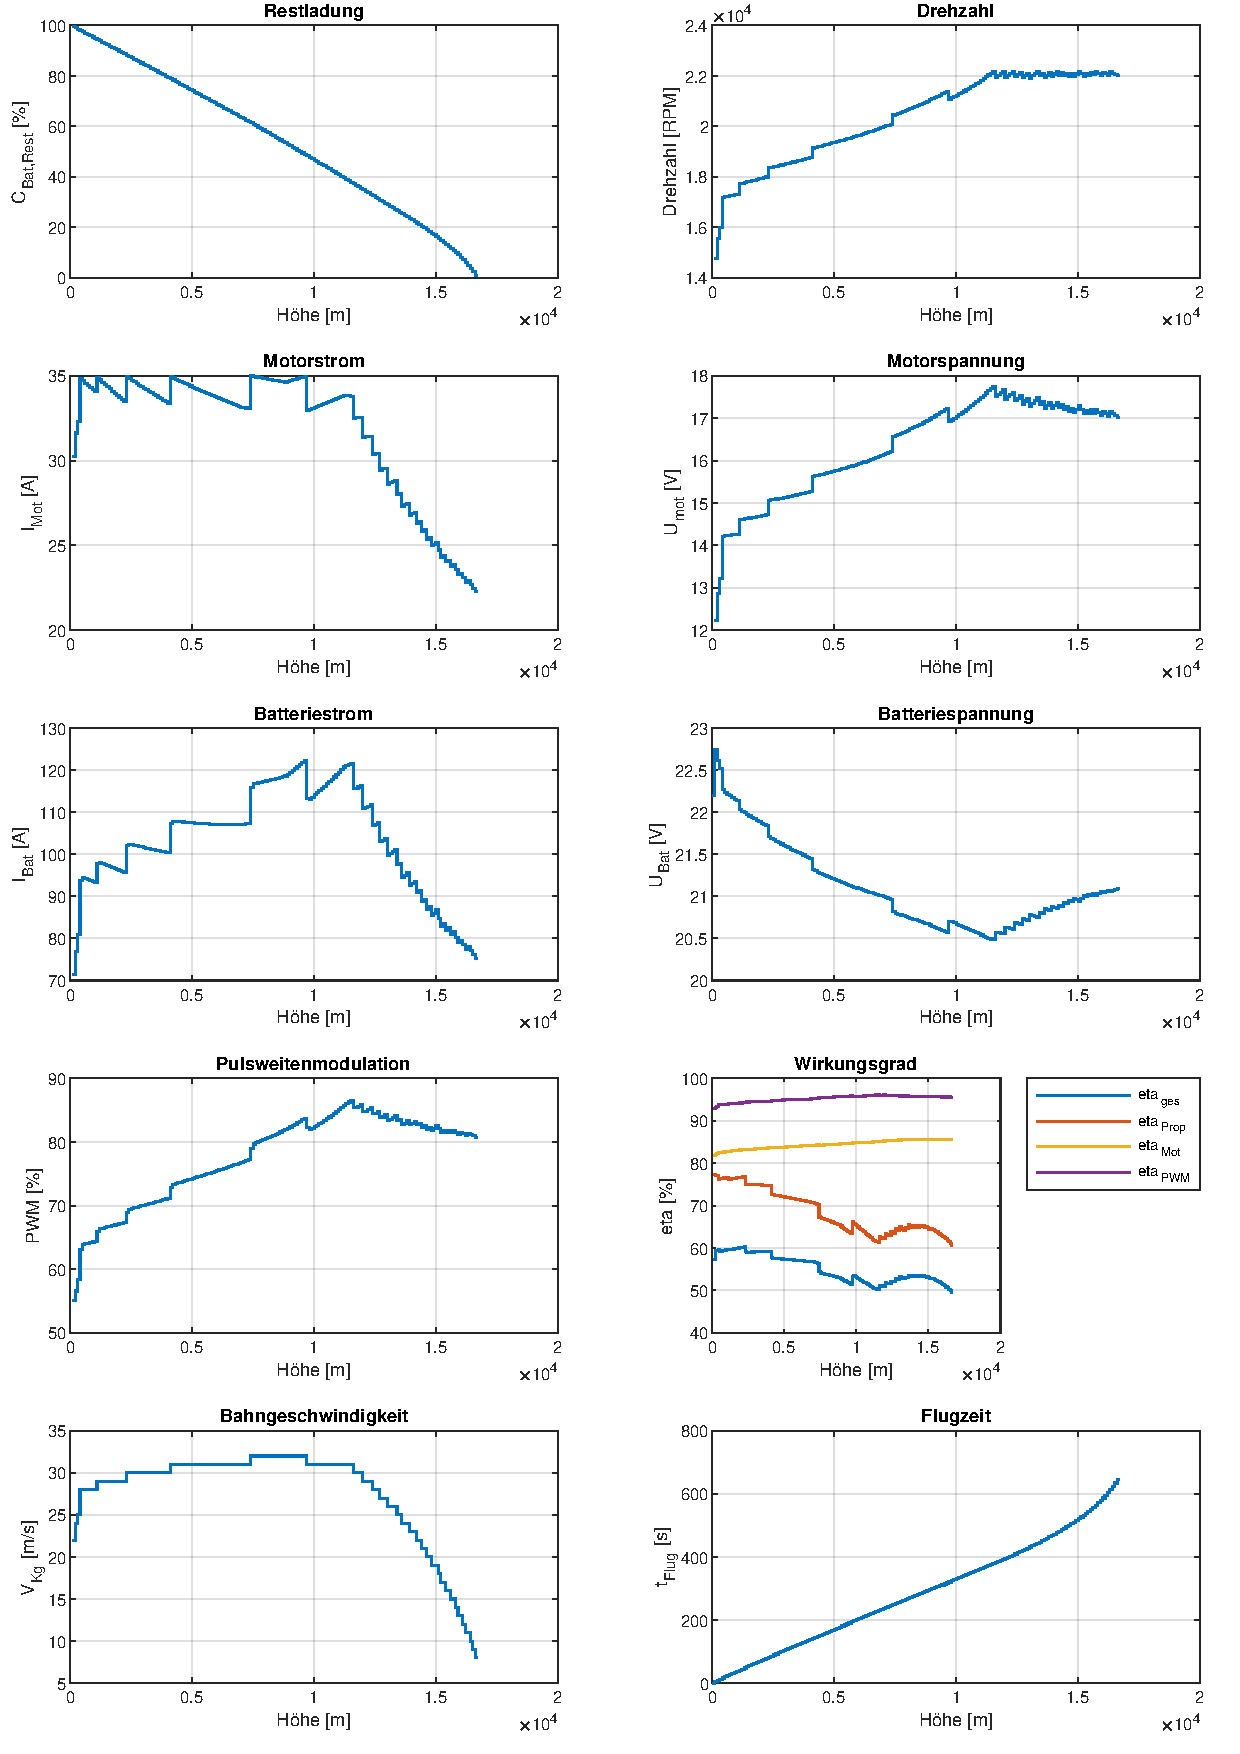
\includegraphics[scale=0.7]{Diagramme/Untersuchung_eta_pwm_halbierung_6.pdf}
	\caption{Leistungsparameter der Multicopter-Referenzkonfiguration (vgl. Tab. \ref{tab:referenzkonfiguration_mulitcopter}) für eine Verbesserung des Motorreglerwirkungsgrades (Halbierung der Verluste) für eine Batterie mit sechs Zellen}
	\label{abb:eta_pwm_6_halb}
\end{figure}

\begin{figure}[H]
\centering
	\includegraphics[scale=0.7]{Diagramme/Untersuchung_eta_pwm_1_6.pdf}
	\caption{Leistungsparameter der Multicopter-Referenzkonfiguration (vgl. Tab. \ref{tab:referenzkonfiguration_mulitcopter}) für eine Verbesserung des Motorreglerwirkungsgrades (keine Verluste) für eine Batterie mit sechs Zellen}
	\label{abb:eta_pwm_6_1}
\end{figure}


\section{Batteriemasse}
\label{sec:batteriemasse}
Es zeigt sich, dass das Optimum des Batteriemassenanteils bei \SI{66.66}{\%} oder leicht darunter liegt. Eine Erhöhung führt zu schlechteren Flugleistungen und einem schnelleren Absinken der Restkapazität gegen Null (vgl. Abb. \ref{abb:batteriemasse_genauer}). Deutlich ist zudem der Einfluss der Batteriemasse auf die Bahngeschwindigkeit gegeben. Mit der Masse sinkt die optimale Bahngeschwindigkeit. 
\begin{figure}[H]
\centering
	\includegraphics[scale=0.7]{Diagramme/Batteriemasse_genauer.pdf}
	\caption{genauere Untersuchung der Batteriemassenabhängigkeit (\ensuremath{m_{Mot}=\SI{106}{g}}, \ensuremath{K_V=\SI{1390}{RPM/V}}, \ensuremath{n_{Prop}=4}, \ensuremath{Propeller=\SI{10x3}{}}, \ensuremath{n_{Bat,cell}=4}, \ensuremath{u_{Wg}=\SI{10}{m/s}})}
	\label{abb:batteriemasse_genauer}
\end{figure}

\section{Verstellpropeller}
\label{sec:vprop_vorgehen}
In Abb. \ref{abb:vpp_vorberechnung} ist die Entnahme aller Kennfelder mit dem vorgegeben Durchmesser dargelegt. Im Anschluss folgt die Flugleistungsberechnung für einen Multicopter mit Verstellpropeller in Abb. \ref{abb:vpp_flugleistungsberechnung}.
\begin{center}
\begin{figure}[H]
\begin{struktogramm}(163,70)
\assign[1]{Multicopter- und Umgebungsparameter festlegen (im Startskript)}
\assign[1]{Diskretisierungen (Geschwindigkeit, Höhe) festlegen}
\assign[1]{Aufruf des Hauptskripts: Leistungsberechnung starten}
\while[5]{Für alle Zeilen der APC-Datenbank}
	\ifthenelse[10]{1}{1}{Stimmt Durchmesser mit dem gesuchten überein?}{ja}{nein}
		\assign[2]{Gehe zur nächsten Zeile}
		\change
		\assign[2]{Lösche Zeile}
	\ifend
\whileend
\while[5]{Für alle Propeller}
	\assign[2]{Extrahiere Propellerkennfeld}
	\assign[2]{Speicher das Ergebnis unter fortlaufenden Nummern}
	\assign[2]{Erhöhe Propellerzähler}
\whileend
\end{struktogramm}
\caption{Programmstruktur für die Entnahme aller Propellerkennfelder mit dem zu untersuchenden Durchmesser}
\label{abb:vpp_vorberechnung}
\end{figure}
\end{center}

\begin{center}
\begin{figure}[H]
\begin{struktogramm}(163,210)
\assign[1]{Initialisierung der Parameterberechnung}
\while[5]{F\"ur alle Höhenabschnitte}
	\assign[1]{H\"ohe, Dichte, Luftdruck Temperatur berechnen}
	\assign[1]{Berechnung des arithmetischen Mittelwertes}
	\assign[1]{Schub- und Leistungskennfeld anpassen}
	\assign[2]{Initialisierung der Leistungsberechnung}
	\while[5]{Für alle Bahngeschwindigkeiten}
		\assign[2]{Initialisierungen}
		\while[5]{Für alle Propeller}
			\assign[2]{\texttt{\textbf{Leistungsberechnung}}}
			\assign[2]{Berechnung benötigter Energiemenge bei dieser Bahngeschwindigkeit mit diesem Propeller}
		\whileend
		\ifthenelse[10]{4}{1}{Sind die Werte NaN?}{nein}{ja}
			\while[5]{Solange Abbruchkriterium nicht erreicht}		
				\assign[2]{Finde den Index mit der geringsten verbrauchten Energiemenge}
				\ifthenelse[10]{1}{1}{Werte innerhalb Leistungsgrenzen?}{ja}{nein}
				\assign[2]{Verlasse Schleife}
				\change
				\assign[2]{Suche nächst kleinere Energiemenge}
				\ifend
			\whileend
			\assign[2]{Übergabe aller Leistungsparameter mit diesem Index}
			\change
			\assign[2]{Verwerfe alle Ergebnisse}
		\ifend
		\assign[2]{Berechne benötigte Energie für Steiggeschwindigkeit}
	\whileend
	\ifthenelse[10]{4}{1}{Sind die Werte NaN?}{nein}{ja}
		\while[5]{Solange Abbruchkriterium nicht erreicht}		
			\assign[2]{Finde den Index mit der geringsten verbrauchten Energiemenge}
			\ifthenelse[10]{1}{1}{Werte innerhalb Leistungsgrenzen?}{ja}{nein}
			\assign[2]{Verlasse Schleife}
			\change
			\assign[2]{Suche nächst kleinere Energiemenge}
			\ifend
		\whileend
		\assign[2]{Übergabe aller Leistungsparameter mit diesem Index}
		\change
		\assign[2]{Verwerfe alle Ergebnisse}
	\ifend
	\assign[2]{Erhöhe Zählervariable}
\whileend
\assign[2]{Ergebnisse der Leistungsparameter in Diagrammen speichern}
\assign[2]{Speichern der Diagramme in .pdf-Datei}
\end{struktogramm}
\caption{Programmstruktur für die Untersuchung des Nutzens eines Verstellpropellers}
\label{abb:vpp_flugleistungsberechnung}
\end{figure}
\end{center}

Der Verlauf des Gesamtwirkungsgrades folgt eindeutig dem Verlauf des Propellerwirkungsgrades. Dieser ist die Ursache für den höheren Gesamtwirkungsgrad des Verstellpropellers (Vgl. Abb. \ref{abb:verstellprop_eta}).

\begin{figure}[H]
\centering
	\includegraphics[scale=0.7]{Diagramme/Verstellprop_eta.pdf}
	\caption{Einfluss des Verstellpropellers auf die maximal erreichbare Höhe mit besonderem Hinblick auf die Einzelwirkungsgrade}
	\label{abb:verstellprop_eta}
\end{figure}

In Abb. \ref{abb:verstellprop_real} ist der Gewichtseinfluss auf die Flugleistungen eines Multicopters mit Verstellpropeller dargestellt. Das Gewicht verringert die Flugleistungen deutlich. Außerdem kann für die Referenzkonfiguration festgehalten werden, dass der Vorteil des Verstellpropellers bei einem Gewicht des Verstellmechanismus von \SI{85}{g} pro Propeller kompensiert wird. Insgesamt ergibt dies einen Anteil von ca. \SI{10}{\%} am Gesamtgewicht. Wird dieser Anteil überschritten, ist der Nutzen des Verstellpropeller nichtig. Alle Gewichtsanteile darunter ergeben einen Nutzen. 
\begin{figure}[H]
\centering
	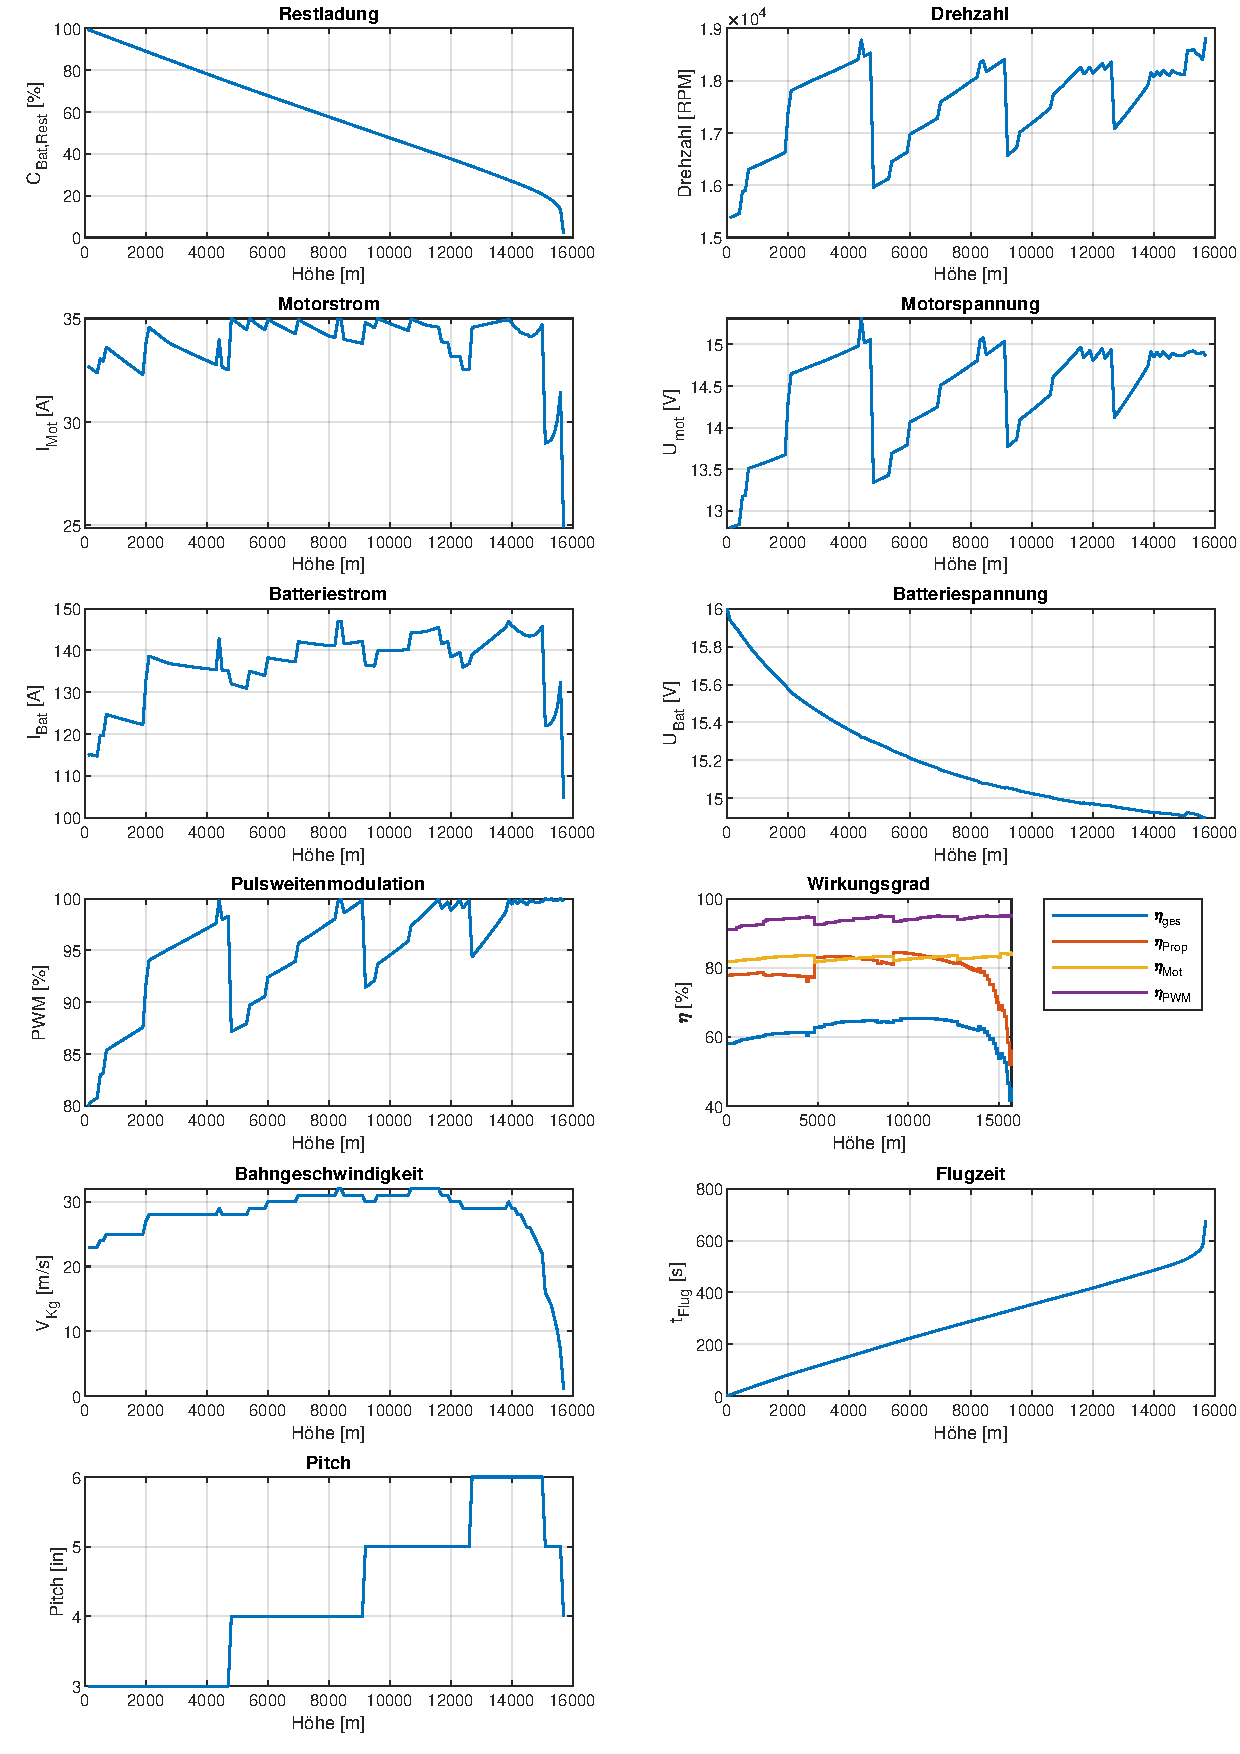
\includegraphics[scale=0.7]{Diagramme/Verstellprop_real.pdf}
	\caption{Einfluss des Verstellpropellers auf die Flugleistungen der Referenzkonfiguration des Multicopters mit einem Gewicht von \SI{85}{g} pro Verstelleinrichtung}
	\label{abb:verstellprop_real}
\end{figure}


\section{Getriebe}
\label{sec:getriebe_vorgehen}
\begin{center}
\begin{figure}[H]
\begin{struktogramm}(163,210)
\assign[1]{Multicopter- und Umgebungsparameter festlegen (im Startskript)}
\assign[1]{Diskretisierungen (Getriebe, Geschwindigkeit, Höhe) festlegen}
\assign[1]{Aufruf des Hauptskripts: Leistungsberechnung starten}
\assign[1]{Initialisierung der Parameterberechnung}
\while[5]{F\"ur alle Höhenabschnitte}
	\assign[1]{H\"ohe, Dichte, Luftdruck Temperatur berechnen}
	\assign[1]{Berechnung des arithmetischen Mittelwertes}
	\assign[1]{Schub- und Leistungskennfeld anpassen}
	\assign[2]{Initialisierung der Leistungsberechnung}
	\while[5]{Für alle Bahngeschwindigkeiten}
		\assign[2]{Initialisierungen}
		\while[5]{Für alle Übersetzungen}
			\assign[2]{\textbf{Leistungsberechnung}}
		\whileend
		\ifthenelse[10]{4}{1}{Sind die Werte NaN?}{nein}{ja}
			\while[5]{Solange Abbruchkriterium nicht erreicht}		
				\assign[2]{Finde den Index mit der geringsten verbrauchten Energiemenge}
				\ifthenelse[10]{1}{1}{Grenzen überschritten?}{nein}{ja}
				\assign[2]{Verlasse Schleife}
				\change
				\assign[2]{Suche nächst kleineren Energiemenge}
				\ifend
			\whileend
			\assign[2]{Übergabe aller Leistungsparameter mit diesem Index}
			\change
			\assign[2]{Verwerfe alle Ergebnisse}
		\ifend
		\assign[2]{Berechne benötigte Energie für Steiggeschwindigkeit}
	\whileend
	\ifthenelse[10]{4}{1}{Sind die Werte NaN?}{nein}{ja}
		\while[5]{Solange Abbruchkriterium nicht erreicht}		
			\assign[2]{Finde den Index mit der geringsten verbrauchten Energiemenge}
			\ifthenelse[10]{1}{1}{Grenzen überschritten?}{nein}{ja}
			\assign[2]{Verlasse Schleife}
			\change
			\assign[2]{Suche nächst kleinere Energiemenge}
			\ifend
		\whileend
		\assign[2]{Übergabe aller Leistungsparameter mit diesem Index}
		\change
		\assign[2]{Verwerfe alle Ergebnisse}
	\ifend
	\assign[2]{Erhöhe Zählervariable}
\whileend
\assign[2]{Ergebnisse der Leistungsparameter in Diagrammen speichern}
\assign[2]{Speichern der Diagramme in .pdf-Datei}
\end{struktogramm}
\caption{Programmstruktur die Untersuchung des Nutzens eines Getriebes}
\label{abb:getriebe_struktogramm}
\end{figure}
\end{center}

\section{Einfluss der Nutzlast}
\label{sec:einfluss_nutzlast}
Auf eine Reduzierung der Batteriemasse durch die zusätzliche Nutzlast wird in Kap. \ref{subsec:aeromet_rb} bewusst verzichtet. Der Vergleich von Abb. \ref{abb:aeromet_rb} mit Abb. \ref{abb:aeromet_rb_batterie_redu} zeigt auf, dass eine Reduzierung der Gesamtmasse im Sinne einer Schubsenkung wenig Einfluss auf die Flugleistungen hat. Dies bestätigt die Aussage aus Abschn. \ref{subsec:groesse}. Der Einfluss der Nutzlast mit konstanten \SI{250}{g} nimmt ab, je kleiner deren Anteil an der Gesamtmasse ist.  

\begin{figure}[H]
\centering
	\includegraphics[scale=0.7]{Diagramme/aeromet_nutzlast_redu.pdf}
	\caption{Einfluss der Batteriemassenreduzierung durch die Nutzlast auf die Flugleistungen der optimalen Lösung (vgl. Tab. \ref{tab:optimale_konfiguration})}
	\label{abb:aeromet_rb_batterie_redu}
\end{figure}



\end{appendix}

%    \newpage
%    \pagenumbering{arabic}
%    \setcounter{page}{\value{page}-1}
%    \setcounter{page}{\value{totalPages}}
\end{document}
% ******************************************************************************
